\documentclass[12pt]{article}

% LaTeX packages
\usepackage{algorithm}
\usepackage{algorithmic}
\usepackage{amsmath}
\usepackage{amssymb}
\usepackage{amsthm}
\usepackage[singlelinecheck=false]{caption}
\usepackage{fullpage}
\usepackage[colorlinks=true,citecolor=blue,linkcolor=blue]{hyperref}
\usepackage{natbib}
\usepackage{thmtools}
\usepackage{tikz}
\usepackage{color}
\usepackage{comment}
\usepackage{commath}
\usepackage{dsfont}
\usepackage{framed}

% TikZ packages
\usetikzlibrary{arrows}
\usetikzlibrary{angles}
\usetikzlibrary{backgrounds}
\usetikzlibrary{calc}
\usetikzlibrary{cd}  % commutative diagrams
\usetikzlibrary{intersections}
\usetikzlibrary{patterns}
\usetikzlibrary{shapes}
\usetikzlibrary{through}

% Math environments
\newtheorem{definition}{Definition}
\newtheorem{proposition}[definition]{Proposition}
\newtheorem{lemma}[definition]{Lemma}
\newtheorem{theorem}[definition]{Theorem}
\newtheorem{corollary}[definition]{Corollary}

% Math symbols and commands
\newcommand{\calF}{\mathcal{F}}
\newcommand{\one}{\mathds{1}}
\newcommand{\R}{\mathbb{R}}  % set of real numbers
\newcommand{\indicator}[1]{\mathbf{1}\left[#1 \right]} % indicator
\newcommand{\ip}[2]{\left\langle #1, #2 \right\rangle} % inner product
\newcommand{\e}{\mathbf{e}}
\newcommand{\zero}{\mathbf{0}}
%\newcommand{\norm}[1]{\left\| #1 \right\|}  % norm of a vector or a matrix
%\DeclareMathOperator*{\deg}{deg}

\DeclareMathOperator*{\argmax}{argmax}
\DeclareMathOperator*{\argmin}{argmin}
\DeclareMathOperator*{\Exp}{\mathbf{E}}  % expected value
\DeclareMathOperator{\diff}{d \!} % differential
\DeclareMathOperator*{\polylog}{polylog}


\definecolor{darkgreen}{rgb}{0,0.5,0}
\definecolor{darkred}{rgb}{0.7,0,0}
\definecolor{teal}{rgb}{0.3,0.8,0.8}
\definecolor{orange}{rgb}{1.0,0.5,0.0}
\definecolor{purple}{rgb}{0.8,0.0,0.8}
\definecolor{blue}{rgb}{0.0,0.0,1.0}
\newcommand{\kibitz}[2]{{\textcolor{#1}{\textsf{\footnotesize #2}}}}
\newcommand{\alina}[1]{\kibitz{darkred}{[AB: #1]}}
\newcommand{\david}[1]{\kibitz{darkgreen}{[DP: #1]}}
\newcommand{\balazs}[1]{\kibitz{purple}{[BS: #1]}}
\newcommand{\deva}[1]{\kibitz{teal}{[DT: #1]}}
\newcommand{\chenyu}[1]{\kibitz{orange}{[CW: #1]}}
\newcommand{\chicheng}[1]{\kibitz{blue}{[CZ: #1]}}


\title{Online Multiclass Linear Classification with Bandit Feedback}

\author{
Alina Beygelzimer \and
D\'avid P\'al \and
Bal\'azs Sz\"or\'enyi \and
Devanathan Thiruvenkatachari \and
Chen-Yu Wei \and
Chicheng Zhang
}

\begin{document}

\maketitle

\begin{abstract}
We study the problem of efficient online multiclass linear classification with
bandit feedback, where all examples belong to one of $K$ classes and lie in the
$d$-dimensional Euclidean space. Previous works have left open the challenge of
designing efficient algorithms with finite mistake bounds when the data is
linearly separable by a margin $\gamma$. In this work, we take a first step
towards this problem. We consider two notions of linear separability: strong
linear separability and weak linear separability.

\begin{enumerate}
\item Under the strong linear separability condition, we design an efficient
algorithm that achieves a near-optimal mistake bound of
$O\left(\frac{K}{\gamma^2} \right)$.

\item Under the more challenging weak linear separability condition, we design
an efficient algorithm with a mistake bound of $2^{\widetilde{O}(\min(K \log^2
\frac{1}{\gamma}, \log K \sqrt{\frac 1 \gamma}))}$ \footnote{We use the notation
$\widetilde{O}(f(\cdot)) = O(f(\cdot) \polylog(f(\cdot)))$.}. Our algorithm is
based on a infinite-dimensional feature mapping that transforms weak linear
separable examples to strong linear separable examples, which in turn is
inspired by \cite{Klivans-Servedio-2008}'s work on learning intersection of
halfspaces.
\end{enumerate}
\end{abstract}

\section{Introduction}
\label{section:introduction}

We study the problem of \textsc{Online Multiclass Linear Classification with
Bandit Feedback}~\citep{Kakade-Shalev-Shwartz-Tewari-2008}. The problem can be
viewed as a repeated game between the learner and the adversary. At each
timestep $t$, the adversary chooses a labeled example $(x_t, y_t)$ where the
feature vector $x_t \in \R^d$ is revealed to the learner and the correct label
$y_t$ is kept secret by the adversary. Upon receiving the feature vector $x_t$,
the learner is asked to make a prediction $\widehat{y}_t$. Immediately after
making its prediction, the learner receives a feedback. In contrast with the
standard full information setting (where the feedback given is the correct label
$y_t$), here the feedback is only a binary indicator of whether the prediction
was correct or not. The protocol of the problem is formally stated below.

\begin{protocol}[h]
\caption{\textsc{Online Multiclass Classification with Bandit Feedback}
\label{algorithm:game-protocol}}
\begin{algorithmic}[1]
{
\REQUIRE{Number of classes $K$, number of rounds $T$.}
\FOR{$t=1,2,\dots,T$}
\STATE Adversary chooses example $(x_t, y_t)$, where $x_t$ is revealed to the learner.
\STATE{Predict class label $\widehat y_t \in \{1,2,\dots,K\}$}
\STATE{Observe feedback $z_t \in \{0,1\}$ \\ \qquad where $z_t = \begin{cases}
0 & \text{if $\widehat y_t = y_t$,} \\
1 & \text{if $\widehat y_t \neq y_t$.}
\end{cases}$
}
\ENDFOR
}
\end{algorithmic}
\end{protocol}

The performance of the learner is measured by its cumulative number of
mistakes $\sum_{t=1}^T z_t = \sum_{t=1}^T \indicator{\widehat y_t \neq y_t}$.
The bandit feedback is a natural feedback model motivated by applications
including online advertising and online content optimization.

In this paper, we focus on the special case when the examples chosen by the
adversary lie in $\R^d$ and are linearly separable with a margin. We introduce
two notions of linear separability, \emph{weak} and \emph{strong}. These are
formally stated in
Definitions~\ref{definition:weak-linear-separability}~and~\ref{definition:strong-linear-separability}.
The standard notion of multiclass linear separability corresponds to the weak
linear separability. For binary classification, the weak and strong separability
are identical. However, they differ for multiclass classification with $K \ge 3$
classes. For multiclass classification with $K$ classes, the standard notion of
linear separability means that the examples from each class lie in an
intersection of $K-1$ halfspaces and the examples outside of the class lie in
the complement of the intersection of the halfspaces. Strong linear separability
means that examples from each class are separated from the remaining examples by
a \emph{single} hyperplane.

In the full-information feedback setting, it is well known that if the examples
have norm at most $R$ and are weakly linearly separable with a margin $\gamma$
then the \textsc{Multiclass Perceptron} algorithm makes at most $\lfloor
2(R/\gamma)^2 \rfloor$ mistakes. This result is very satisfying since the upper
bound on the number of mistakes is information-theoretically optimal and at the
same time the \textsc{Multiclass Perceptron} algorithm has low time and memory
complexity.

The bandit feedback setting, however, is much more challenging. For the case
when the examples are strongly linearly separable, we design a simple and
efficient algorithm with an expected number of mistakes at most $(K-1) \lfloor
4(R/\gamma)^2 \rfloor$. The algorithm can be viewed as running $K$ copies of the
\textsc{Binary Perceptron} algorithm, one copy for each class. Intuitively
speaking, the factor $K-1$ is the price we pay for the bandit feedback, or more
precisely, the lack of full-information feedback. We also prove that any
(possibly randomized) algorithm makes $\Omega(K (R/\gamma)^2))$ mistakes in the
worst case.

For the case when examples are weakly linearly separable, we construct a feature
mapping $\phi$ such that makes them \emph{strongly} linearly separable. We then
use the kernelized version of the algorithm for the strongly separable case; for
more details on kernel methods see e.g.~\citet{Scholkopf-Smola-2002} and
\citet{Shawe-Taylor-Cristianini-2004}. The kernel $k(x,y)$ corresponding to the
feature mapping $\phi$ has a simple explicit formula and can be computed in
$O(d)$ time.

The number of mistakes of the kernelized algorithm depends on the margin in the
corresponding feature space. We analyze how the margin parameter of weak
separability in the original space $\R^d$ gets transformed into a margin
parameter of strong separability in the new feature space. This problem is
related to the problem of learning intersection of halfspaces and has been
studied previously by \citet{Klivans-Servedio-2008}. In fact, our analysis can
be viewed as a follow up on their work. We improve on the results of
\citet{Klivans-Servedio-2008} by removing the dependency on the original
dimension $d$.

The resulting kernelized algorithm runs in time that is polynomial in the
original dimension of the feature vectors $d$, the number of classes $K$, and
the number of rounds $T$. We prove that if the examples lie in unit ball of
$\R^d$ and are weakly separable with margin $\gamma$, the algorithm makes at
most $O(???)$ mistakes.

\section{Related work}
\label{section:related-work}
The problem of bandit multiclass linear classification is initially formulated
 by the pioneering work of~\cite{Kakade-Shalev-Shwartz-Tewari-2008}. In that work,
 two computationally
 inefficient algorithms that work in the $\gamma$-weak linearly separable setting are proposed: one with a mistake bound of
 $O(k^2 d \ln(\frac{d}{\gamma^2}))$, the other with a mistake bound of $\tilde{O}(\frac{k^2}{\gamma^2} \ln T)$.
 In addition, the authors propose the Banditron algorithm, a computationally efficient
 algorithm that has a $O(T^{2/3})$ regret in the general setting, and has a
 $O(\sqrt{T})$ mistake bound in the $\gamma$-weak linearly separable setting.
The polynomial dependence of Banditron's mistake bound on the time horizon is undesirable
for problems with a long time horizon.
 One key open question left by~\cite{Kakade-Shalev-Shwartz-Tewari-2008} is whether
 one can deesign computationally efficient algorithms that achieve mistake bounds that match or improve over those of inefficient algorithms.
 In this paper, we take a step towards answering this question, showing that
 efficient algorithms with mistake bounds quasipolynomial in the margin parameter can be obtained.

 %Whether one can design an efficient algorithm with a
 %finite mistake bound that has no dimensionality dependence is mentioned as an open problem in
 %~\cite{Kakade-Shalev-Shwartz-Tewari-2008}, where in this paper we provide a positive answer.
 %$O(k^2 d \ln(\frac{d}{\gamma^2}))$

Many works consider bandit multiclass classification in the general non-separable setting.
\cite{Abernethy-Rakhlin-2009} poses the open problem of whether one can design
and efficient algorithm to get a $O(\sqrt{T})$ regret against some reasonable loss functions.
\cite{CrammerG13} shows that such an algorithm can be obtained, under the assumption that the distribution of the label $y$ conditioned on feature $x$ satisfies certain parametric noise assumption.
\cite{Hazan-Kale-2011} developed the Newtron algorithm, which has a regret
between $O(\ln T)$ and $O(T^{2/3})$ against the multiclass logistic loss, where the exact order of the regret depends on the diameter of the benchmark class. In particular, if the diameter is $O(\ln T)$, its regret bound would become
$O(T^{2/3})$.
The SOBA algorithm by \cite{Beygelzimer-Orabona-Zhang-2017} achieves a regret of $\tilde{O}(\sqrt{T})$ against the $\eta$-loss~\cite{Orabona-Cesa-Bianchi-Gentile-2012}; in addition, their regret bound does not depend sensitively on the diameter of the benchmark class.
\cite{Foster-Kale-Luo-Mohri-Sridharan-2018} developed an algorithm that has a regret of $\tilde{O}(\sqrt{T})$ against the multiclass logistic loss, where it doubly-exponentially improves over \cite{Hazan-Kale-2011}'s regret on its dependence on the diameter of the benchmark class.
Recently, \cite{Foster-Krishnamurthy-2018} developed a rich theory on contextual bandits with surrogate losses, focusing on benchmarks of the form $\min_{f \in \calF} \frac 1 K \sum_{i=1}^K \phi( f_i(x) )$, where $\calF$ contains function $f$ such that $\sum_{i=1}^K f_i(\cdot) \equiv 0$,
and $\phi(s) = \max(1 - \frac s \gamma, 0)$ and $\min(1, \max(1 - \frac s \gamma, 0))$.
On one hand, it gives information-theoretic mistake upper bounds under various settings of $\calF$, for instance parametric and nonparametric classes; On the other hand, it gives an efficient algorithm that has a $O(\sqrt{T})$ regret against the benchmark of $\calF = \cbr{x \mapsto W x: W \in \R^{k \times d}, \one^T W = 0}$.

\cite{Chen-Lin-Lu-2014, Zhang-Jung-Tewari-2018} study online bandit multiclass boosting under bandit feedback, where one can view online boosting as online linear classification by treating each base hypothesis as a separate feature.
\cite{Chen-Lin-Lu-2014}'s online weak learning condition implies that there is a convex combination of base hypotheses that one-versus-all separates all examples with a margin. Under this condition, it gives an algorithm with a $O(T^{3/4})$ mistake bound.
\cite{Zhang-Jung-Tewari-2018} considers an online weak learning condition that implies that there is a convex combination of base hypotheses that weakly separates all examples with a margin (See~\cite{Mukherjee-Schapire-2013}, Theorem 3). Under this condition, it gives an algorithm with a $O(\sqrt{T})$ mistake bound with the knowledge of the edge parameter; in addition, it gives an adaptive algorithm with a $O(T^{3/4})$ mistake bound.


%\cite{Chen-Chen-Zhang-Chen-Zhang-2009} studies the approach of reducing bandit multiclass learning to online binary classification using one-versus-all reduction. They show that

%Their results do not imply a finite mistake bound in the weakly separable setting, in that the benchmark loss can still be $\Omega(T)$.


%\begin{itemize}
%\item \cite{Abernethy-Rakhlin-2009}

%\item \cite{Chen-Chen-Zhang-Chen-Zhang-2009}

%\item \cite{Hazan-Kale-2011}

%\item \cite{Beygelzimer-Orabona-Zhang-2017}

%\item \cite{Foster-Kale-Luo-Mohri-Sridharan-2018}

%\item \cite{Foster-Krishnamurthy-2018}
%\end{itemize}

%TODO

\section{Notions of linear separability}
\label{section:notions-of-linear-separability}

We define two notions of linear separability for multiclass classification. The
first notion is the standard notion of linear separability used in the proof of
the mistake bound for the \textsc{Multiclass Perceptron} algorithm. The second
notion is stronger, i.e. more restrictive. However, it is more suitable for the
bandit setting, since it allows for a simple and efficient algorithm; see
Section~\ref{section:algorithm-for-strongly-linearly-separable-data}.

\begin{definition}[Weak linear separability]
\label{definition:weak-linear-separability}
Let $(V,\ip{\cdot}{\cdot})$ be an inner product space, $K$ be a positive
integer, and $\gamma$ be a positive real number. Let $(x_1, y_1), (x_2,
y_2), \dots, (x_T, y_T)$ be labeled examples in $V \times \{1,2,\dots,K\}$.

The examples are said to be \emph{weakly linearly separable with a
margin $\gamma$} if there exist vectors $w_1, w_2, \dots, w_K \in V$ such
that
\begin{align}
\label{equation:weak-linear-separability-1}
& \sum_{i=1}^K \norm{w_i}^2 \le 1 \; , \\
\label{equation:weak-linear-separability-2}
& \begin{gathered}
\forall t \in \{1,2,\dots,T\} \quad \forall i \in \{1,2,\dots, K\} \setminus \{y_t\} \\
\ip{x_t}{w_{y_t}} \ge \ip{x_t}{w_i} + \gamma \; .
\end{gathered}
\end{align}
\end{definition}

\begin{definition}[Strong linear separability]
\label{definition:strong-linear-separability}
Let $(V,\ip{\cdot}{\cdot})$ be an inner product space, $K$ be a positive
integer, and $\gamma$ be a positive real number. Let $(x_1, y_1), (x_2,
y_2), \dots, (x_T, y_T)$ be labeled examples in $V \times \{1,2,\dots,K\}$.

The examples are said to be \emph{strongly linearly separable with a
margin $\gamma$} if there exist vectors $w_1, w_2, \dots, w_K \in V$ such
that
\begin{align}
\label{equation:strong-linear-separability-1}
& \sum_{i=1}^K \norm{w_i}^2 \le 1 \; , \\
\label{equation:strong-linear-separability-2}
& \forall t \in \{1,2,\dots,T\} \qquad \qquad \ip{x_t}{w_{y_t}} \ge \frac \gamma 2 \; , \\
\label{equation:strong-linear-separability-3}
& \begin{gathered}
\forall t \in \{1,2,\dots,T\} \qquad \forall i \in \{1,2,\dots, K\} \setminus \{y_t\} \\
\ip{x_t}{w_i} \le - \frac \gamma 2 \; .
\end{gathered}
\end{align}
\end{definition}

The notion of weak linear separability with a margin is standard. It is used in
the full-information setting to upper bound the number of mistakes of the
\textsc{Multiclass Perceptron} algorithm. It is a folklore result that if a set
of labeled examples is separable with a margin $\gamma$ and the norm of the
examples is bounded by $R$, then \textsc{Multiclass Perceptron} algorithm makes
at most $\left\lfloor 2(R/\gamma)^2 \right \rfloor$ mistakes. Another folklore
result is that \textsc{Multiclass Perceptron} is essentially optimal in the
sense that any deterministic algorithm must make $\left\lfloor (R/\gamma)^2
\right \rfloor$ mistakes in the worst case. For completeness, we state the
\textsc{Multiclass Perceptron} algorithm and give proofs of both of these
results in Appendix~\ref{section:multiclass-perceptron-proofs}.

The notion of strong linear separability has appeared in the literature; see
e.g.~\citet{Chen-Chen-Zhang-Chen-Zhang-2009}.
Intuitively, strong linear
separability means that, for each class $i$, the set of examples belonging to
class $i$ and the set of example belonging to the remaining $K-1$ classes are
separated by a linear classifier $w_i$ by a margin $\frac \gamma 2$.

It is easy to see that if a set of labeled examples are strongly linearly
separable with margin $\gamma$, then they are weakly linearly separable with
the same margin. Indeed, if $w_1, w_2, \dots, w_K \in V$
satisfy \eqref{equation:strong-linear-separability-1},
\eqref{equation:strong-linear-separability-2},
\eqref{equation:strong-linear-separability-3} then they satisfy
\eqref{equation:weak-linear-separability-1} and
\eqref{equation:weak-linear-separability-2}.

In the special case of $K=2$, if a set of labeled examples are weakly linearly
separable with a margin $\gamma$, then they are strongly linearly separable with
the same margin. Indeed, if $w_1, w_2$ satisfy
\eqref{equation:weak-linear-separability-1} and
\eqref{equation:weak-linear-separability-2} then $w_1' = \frac{w_1 - w_2}{2}$,
$w_2' = \frac{w_2 - w_1}{2}$ satisfy
\eqref{equation:strong-linear-separability-1},
\eqref{equation:strong-linear-separability-2},
\eqref{equation:strong-linear-separability-3}. The first condition follows from
$\norm{w_i'}^2 \le (\frac{1}{2} \norm{w_1} + \frac{1}{2} \norm{w_2})^2 \le
\frac{1}{2}\norm{w_1}^2 + \frac{1}{2}\norm{w_2}^2 \le \frac{1}{2}$ for $i=1,2$.
The last two condition follows from the fact that $w_1' - w_2' = w_1 - w_2$.

However, for any $K \ge 3$ and any inner product space of dimension at least
$2$, there exists a set of labeled examples that is weakly linearly separable
with a positive margin $\gamma$ but it is not strongly linearly separable with
any positive margin $\gamma$. An example of such set of labeled examples is
shown in~\autoref{figure:weakly-linearly-separable-examples-with-margin}.

\begin{figure}
\begin{center}
\input{figures/weakly-linearly-separable-examples-with-margin}
\end{center}
\caption[]{A set of labeled examples in $\R^2$. The examples belong to
$K=3$ classes colored white, gray and black respectively. Each class lies in a
$120^\circ$ wedge. In other words, each class lies in an intersection of two
halfspaces.
\chicheng{Do we have an explicit formula for $W$ in this example? It might help
to provide it.}

While the examples are weakly linearly separable with a positive margin
$\gamma$, they are \emph{not} strongly linearly separable with any positive
margin $\gamma$. For instance, there do not exist linear separators that
separates the examples belonging to the gray class from the examples belonging
to the remaining two classes.
}
\label{figure:weakly-linearly-separable-examples-with-margin}
\end{figure}

\section{Algorithm for strongly linearly separable data}
\label{section:algorithm-for-strongly-linearly-separable-data}

In this section, we present an algorithm for \textsc{Online Multiclass
Classification with Bandit Feedback} and prove an upper bound on the number of
mistakes under the assumption that the examples are strongly linearly separable
with a margin. The algorithm is stated as
Algorithm~\ref{algorithm:algorithm-for-strongly-linearly-separable-examples} and
the mistake upper bound is stated as
\autoref{theorem:strongly-separable-example-mistake-upper-bound}.

The idea behind the algorithm is to use $K$ copies of the \textsc{Binary
Perceptron} algorithm, where each copy corresponds to a class.
In each round, copy $i$
makes a binary prediction, indicating whether the example belongs to class $i$ or not.
If at least one copy makes a positive prediction, the algorithm
chooses its prediction as one of the classes corresponding to a positive prediction.
If all copies make negative
predictions, the algorithms makes a prediction uniformly at random.

%accordingly. If multiple copies make positive predictions, the
%algorithm chooses one of them arbitrarily

\begin{algorithm}[h]
\caption{\textsc{Bandit Algorithm for Strongly Linearly Separable Examples}
\label{algorithm:algorithm-for-strongly-linearly-separable-examples}}
\begin{algorithmic}[1]
{
\REQUIRE{Number of classes $K$.}
\REQUIRE{Number of rounds $T$.}
\REQUIRE{Inner product space $(V,\ip{\cdot}{\cdot})$.}
\STATE{Initialize $w_1^{(1)} = w_2^{(1)} = \dots = w_K^{(1)} = 0$}
\FOR{$t=1,2,\dots,T$}
\STATE{Observe feature vector $x_t \in V$}
\STATE{Compute $S_t = \left\{ i ~:~ 1 \le i \le K, \ \ip{w_i^{(t)}}{x_t} \ge 0 \right\}$}
\IF{$S_t = \emptyset$}
\STATE{Predict $\widehat y_t \sim \text{Uniform}(\{1,2,\dots,K\})$}
\STATE{Observe feedback $z_t \in \{0,1\}$ \\ \qquad where $z_t = \indicator{\widehat y_t \neq y_t}$}
\IF{$z_t = 1$}
\STATE{Set $w_i^{(t+1)} = w_i^{(t)}$ for all $i \in \{1,2,\dots,K\}$}
\ELSE
\STATE{Set $w_i^{(t+1)} = w_i^{(t)}$ \\ \qquad  for all $i \in \{1,2,\dots,K\} \setminus \{\widehat y_t\}$}
\STATE{Update $w_{\widehat y_t}^{(t+1)} = w_{\widehat y_t}^{(t)} + x_t$}
\label{line:pos-update}
\ENDIF
\ELSE
\STATE{Predict $\widehat y_t \in S_t$ chosen arbitrarily}
\STATE{Observe feedback $z_t \in \{0,1\}$ \\ \qquad where $z_t = \indicator{\widehat y_t \neq y_t}$}
\IF{$z_t = 1$}
\STATE{Set $w_i^{(t+1)} = w_i^{(t)}$ \\ \qquad for all $i \in \{1,2,\dots,K\} \setminus \{\widehat y_t\}$}
\STATE{Update $w_{\widehat y_t}^{(t+1)} = w_{\widehat y_t}^{(t)} - x_t$}
\label{line:neg-update}
\ELSE
\STATE{Set $w_i^{(t+1)} = w_i^{(t)}$ for all $i \in \{1,2,\dots,K\}$}
\ENDIF
\ENDIF
\ENDFOR
}
\end{algorithmic}
\end{algorithm}

\begin{theorem}[Mistake upper bound]
\label{theorem:strongly-separable-example-mistake-upper-bound}
Let $(V, \ip{\cdot}{\cdot})$ be an inner product space, $K$ be a positive
integer, $\gamma$ be a positive real number, $R$ be a non-negative real number. If
$(x_1, y_1), (x_2, y_2), \dots, (x_T, y_T)$ is a sequence of labeled examples in
$V \times \{1,2,\dots,K\}$ such that
\begin{enumerate}
  \item the examples are strongly linearly separable with margin $\gamma$ (Definition~\ref{definition:strong-linear-separability}),
  \item $\norm{x_1}, \norm{x_2}, \dots, \norm{x_T} \le R$,
\end{enumerate}
then the
expected number of mistakes
Algorithm~\ref{algorithm:algorithm-for-strongly-linearly-separable-examples}
makes is at most $(K-1) \lfloor 4(R/\gamma)^2 \rfloor$.
\end{theorem}

\begin{proof}
Let $M = \sum_{t=1}^T z_t$ be the number of
mistakes Algorithm~\ref{algorithm:algorithm-for-strongly-linearly-separable-examples} makes.
Let $A
= \sum_{t ~:~ S_t \neq \emptyset} z_t$ be the number of mistakes in the rounds
when $S_t \neq \emptyset$ and let $B = \sum_{t ~:~ S_t = \emptyset} z_t$ be the
number of mistakes in the rounds when $S_t = \emptyset$.
It can be easily seen that $M = A + B$. %We now upper bound $A$ and $B$ separately.

Let $C$ be the number of times line~\ref{line:pos-update} gets executed. Let $U$ be the number of
times line~\ref{line:pos-update} and line~\ref{line:neg-update} get executed. In other words, $U$ is the number of
times the $K$-tuple of vectors $(w_1^{(t)}, w_2^{(t)}, \dots, w_K^{(t)})$ gets
updated. It can be easily seen that $U = A + C$.

The key observation is that $\Exp[B] = (K-1) \Exp[C]$. The equality holds
because if $S_t = \emptyset$, there is $1/K$ probability that the algorithm
guesses the correct label and with probability $(K-1)/K$ algorithm's guess is
incorrect. Putting all the information together, we get that
\begin{align}
\Exp[M]
& = \Exp[A] + \Exp[B] \nonumber \\
& = \Exp[A] + (K-1) \Exp[C] \nonumber \\
& \le (K-1) \Exp[A + C] \nonumber\\
& = (K-1) \Exp[U]  \; .
\label{eqn:mistake-update}
\end{align}

To finish the proof, we need to upper bound the number of updates $U$. We claim
that $U \le \lfloor (R/\gamma)^2 \rfloor$. The proof of this upper bound is
similar to the proof of the mistake bound for \textsc{Multiclass Perceptron}
algorithm. Let $w_1^*, w_2^*, \dots, w_K^* \in V$ be vectors that satisfy
\eqref{equation:strong-linear-separability-1},
\eqref{equation:strong-linear-separability-2} and
\eqref{equation:strong-linear-separability-3}.
The $K$-tuple $(w_1^{(t)}, w_2^{(t)}, \dots, w_K^{(t)})$
changes only if there is an update in round $t$.
We investigate how $\sum_{i=1}^K \norm{w_i^{(t)}}^2$ and
$\sum_{i=1}^K \ip{w_i^*}{w_i^{(t)}}$ change. If there is an update in round $t$,
by lines~\ref{line:pos-update} and~\ref{line:neg-update}, we always have
$ w_{\widehat y_t}^{(t+1)} = w_{\widehat y_t}^{(t)} + (-1)^{z_t} x_t $,
and for all $i \neq \widehat y_t$, $w_{i}^{(t+1)} = w_{i}^{(t)}$.
Therefore,
\begingroup
\allowdisplaybreaks
\begin{align*}
& \sum_{i=1}^K \norm{w_i^{(t+1)}}^2 \\
& = \left( \sum_{i \in \{1,2,\dots,K\} \setminus \{\widehat y_t\}} \norm{w_i^{(t)}}^2 \right) + \norm{w_{\widehat y_t}^{(t+1)}}^2 \\
& = \left( \sum_{i \in \{1,2,\dots,K\} \setminus \{\widehat y_t\}} \norm{w_i^{(t)}}^2 \right) + \norm{w_{\widehat y_t}^{(t)} + (-1)^{z_t} x_t}^2 \\
& = \left( \sum_{i=1}^K \norm{w_i^{(t)}}^2 \right) + \norm{x_t}^2 + \underbrace{(-1)^{z_t} 2 \ip{w_{\widehat y_t}^{(t)}}{x_t}}_{\le 0} \\
& \le \left( \sum_{i=1}^K \norm{w_i^{(t)}}^2 \right) + \norm{x_t}^2 \\
& \le \left( \sum_{i=1}^K \norm{w_i^{(t)}}^2 \right) + R^2 \; .
\end{align*}
\endgroup
Hence, after $U$ updates,
\begin{equation}
\sum_{i=1}^K \norm{w_i^{(T+1)}}^2 \le R^2 U \; .
\label{eqn:norm-ub}
\end{equation}
Similarly, if there is an update in round $t$, we have
\begin{align*}
& \sum_{i=1}^K \ip{w_i^*}{w_i^{(t)}} \\
& = \left( \sum_{i \in \{1,2,\dots,K\} \setminus \{\widehat y_t\}} \ip{w_i^*}{w_i^{(t)}} \right) + \ip{w_{\widehat y_t}^*}{w_{\widehat y_t}^{(t+1)}} \\
& = \left( \sum_{i \in \{1,2,\dots,K\} \setminus \{\widehat y_t\}} \ip{w_i^*}{w_i^{(t)}} \right) \\
& \qquad + \ip{w_{\widehat y_t}^*}{w_{\widehat y_t}^{(t)} + (-1)^{z_t} x_t} \\
& = \left( \sum_{i=1}^K \ip{w_i^*}{w_i^{(t)}} \right) + (-1)^{z_t} \ip{w_{\widehat y_t}^*}{x_t} \\
& \ge \left( \sum_{i=1}^K \ip{w_i^*}{w_i^{(t)}} \right) + \frac \gamma 2,
\end{align*}
where the last inequality follows from a case analysis on $z_t$ and
Definition~\ref{definition:strong-linear-separability}: if $z_t = 0$, then
$\widehat y_t = y_t$, by Equation~\eqref{equation:strong-linear-separability-2}, we have
that $\ip{w_{\widehat y_t}^*}{x_t} \geq \frac \gamma 2$;
if $z_t = 1$, then $\widehat y_t \neq y_t$, by Equation~\eqref{equation:strong-linear-separability-3},
we have that $\ip{w_{\widehat y_t}^*}{x_t} \leq -\frac \gamma 2$.

%\eqref{equation:strong-linear-separability-2}
%and \eqref{equation:strong-linear-separability-3} and analysis of the cases $z_t = 0$ and $z_t = 1$.

Thus, after $U$ updates,
\begin{equation}
\sum_{i=1}^K \ip{w_i^*}{w_i^{(T+1)}} \ge \frac {\gamma U} 2 \; .
\label{eqn:norm-lb}
\end{equation}
Applying Cauchy-Schwartz's inequality twice, and using assumption
\eqref{equation:strong-linear-separability-1}, we get that
\begin{align*}
\sum_{i=1}^K \ip{w_i^*}{w_i^{(T+1)}}
& \le \sum_{i=1}^K \norm{w_i^*} \cdot \norm{w_i^{(T+1)}} \\
& \le \sqrt{\sum_{i=1}^K \norm{w_i^*}^2} \sqrt{\sum_{i=1}^K \norm{w_i^{(T+1)}}^2} \\
& \le \sqrt{\sum_{i=1}^K \norm{w_i^{(T+1)}}^2} \; .
\end{align*}
Combining the above inequality with Equations~\eqref{eqn:norm-ub} and~\eqref{eqn:norm-lb}, we get
$$
(\frac{\gamma U}{2})^2 \le \sum_{i=1}^K \norm{w_i^{(T+1)}}^2 \le R^2 U \; .
$$
We conclude that $U \le 4(R/\gamma)^2$. Since $U$ is an integer, $U \le \lfloor 4(R/\gamma)^2 \rfloor$.

Applying Equation~\eqref{eqn:mistake-update}, we get
\[ \Exp[M] \leq (K-1) \Exp[U] \leq (K-1) \lfloor 4(R/\gamma)^2 \rfloor. \qedhere \]
\end{proof}

The upper bound $(K-1) \lfloor 4(R/\gamma)^2 \rfloor$ on the expected number of
mistakes of
Algorithm~\ref{algorithm:algorithm-for-strongly-linearly-separable-examples} is
optimal to within constant factor as long as the number of classes $K$ is
at most $O((R/\gamma)^2)$. This is proved in
\autoref{theorem:strongly-separable-example-mistake-lower-bound} below.

\begin{theorem}[Mistake lower bound]
\label{theorem:strongly-separable-example-mistake-lower-bound}
Let $\gamma$ be a positive real number, and $R$ be a non-negative real
number. For any (possibly randomized) algorithm $\calA$ for the \textsc{Online
Multiclass Classification with Bandit Feedback} with $K \le
(R/\gamma)^2$ classes there exists an inner product space $(V,
\ip{\cdot}{\cdot})$, a non-negative integer $T$ and a sequence of labeled
examples $(x_1, y_1), (x_2, y_2), \dots, (x_T, y_T)$ in $V \times
\{1,2,\dots,K\}$ that are strongly linearly separable with margin $\gamma$, the
norms satisfy $\norm{x_1}, \norm{x_2}, \dots, \norm{x_T} \le R$ and the expected
number of mistakes $\calA$ makes is at least $\frac{K-1}{2} \left\lfloor
\frac{1}{4} (R/\gamma)^2 \right\rfloor$.
\end{theorem}

\paragraph{Remark.} Irrespective of any conditions on $K$, $R$, and $\gamma$, a trivial lower bound
on the expected number of mistakes of any randomized algorithm is
$\frac{K-1}{2}$. (Adversary chooses the same example over and over.) However, it
is unclear if the trivial lower bound is the best possible if $K$ is large,
i.e., $\omega((R/\gamma)^2)$. We leave this as an open problem.

\begin{proof}
We use probabilistic method. Let $M = \left\lfloor \frac{1}{4} (R/\gamma)^2
\right\rfloor$. Let $V = \R^{M+1}$ equipped with the standard inner product.
Let $e_1, e_2, \dots, e_{M+1}$ be the standard orthonormal basis of $V$. We
define vectors $v_1, v_2, \dots, v_M \in V$ where $v_j = \frac{R}{\sqrt{2}}(e_j
+ e_{M+1})$ for $j=1,2,\dots,M$. Let $\ell_1, \ell_2, \dots, \ell_M$ be chosen
i.i.d. uniformly at random from $\{1,2,\dots,K\}$ and independently of any
randomness used the by algorithm $\calA$. Let $T = M (K - 1)$. We define examples $(x_1,
y_1), (x_2, y_2), \dots, (x_T, y_T)$ as follows. For any $j=1,2,\dots,M$ and any
$h=1,2,\dots,K-1$,
$$
(x_{(j-1)(K-1) + h}, y_{(j-1)(K-1) + h}) = (v_j, \ell_j)
$$


With probability one, the norm of each example is exactly $R$.
We show that with probability
one, the examples are strongly separable with margin $\gamma$. To see
that, consider $w_1^*, w_2^*, \dots, w_K^* \in V$ defined by
$$
w_i^* = \sqrt{2} \frac{\gamma}{R} \left( \sum_{j ~:~ \ell_j = i} e_j \right) - \frac{\sqrt{2}}2 \frac{\gamma}{R} e_{M+1}
$$
for $i=1,2,\dots,K$.

for $i \in \{1,2,\dots,K\}$ and any $j \in
\{1,2,\dots,M\}$, we consider the inner product of $w_i^*$ and $v_j$.
If $i = \ell_j$, $\ip{w_i^*}{v_j} = \gamma - \frac \gamma 2 = \frac \gamma 2$;
otherwise $i \neq \ell_j$, in this case,
$\ip{w_i^*}{v_j} = 0 - \frac \gamma 2 = - \frac \gamma 2$.
This means that $w_1^*, w_2^*, \dots, w_K^*$ satisfy
conditions
\eqref{equation:strong-linear-separability-2} and
\eqref{equation:strong-linear-separability-3}. Condition \eqref{equation:strong-linear-separability-1}
is satisfied since
\begin{multline*}
\sum_{i=1}^K \norm{w_i^*}^2
= 2 \frac{\gamma^2}{R^2} \sum_{j=1}^M \norm{e_j}^2 +  \frac{\gamma^2}{2 R^2} K \norm{e_{M+1}}^2 \\
= 2 \frac{\gamma^2}{R^2} M + \frac{\gamma^2}{2 R^2} K
\le \frac{1}{2} + \frac{1}{2}
= 1 \; .
\end{multline*}

It remains to lower bound the expected number of mistakes of $\calA$. For
any $j \in \{1,2,\dots,M\}$, consider the expected number of mistakes the
algorithm makes in rounds $(K-1)(j-1) + 1, (K-1)(j-1) + 2, \dots, (K-1)j$.

Define a filtration $\cbr{\calB_j}_{j=0}^M$,
where $\calB_j = \sigma((x_1, y_1), \ldots, (x_{(K-1)j}, y_{(K-1)j}))$
for every $j$ in $\{1,2,\dots,M\}$.
By Claim 2 of~\cite{Daniely-Helbertal-2013}, as $\ell_j$
is chosen uniformly from $\cbr{1,\ldots,K}$ and independent of $\calB_{j-1}$,
\[ \Exp \sbr{ \sum_{t=(K-1)(j-1) + 1}^{(K-1)j} z_t \Bigg| \calB_{j-1} } \geq \frac{K-1}2. \]
This implies that
\[ \Exp \sbr{ \sum_{t=(K-1)(j-1) + 1}^{(K-1)j} z_t } \geq \frac{K-1}2. \]
Summing over all $j$ in $\{1,2,\dots,M\}$,
\[ \Exp \sbr{ \sum_{t=1}^{(K-1)M} z_t} \geq \frac{K-1}2 \cdot M = \frac{K-1}2 \left\lfloor \frac 1 4 (R/\gamma)^2 \right\rfloor. \]

%In these rounds,
%the algorithm is guessing the label $\ell_j$. Since $\ell_j$ is chosen uniformly
%at random from the set $\{1,2,\dots,K\}$ and feedback is only binary, the
%expected number of mistakes the algorithm makes in these rounds is at least
%$\frac{K-1}{2}$. Altogether, the algorithm makes at least $\frac{K-1}{2} M$
%mistakes in expectation.

%\chicheng{I think this part need to be formalized, by directly using
%~\cite{Daniely-Helbertal-2013}, Claim 2.}
%Can we assume without loss of generality
%that a deterministic prediction algorithm will have a smaller expected cost?
%If so, define $F(k)$ be the number of mistake that will be made by the algorithm,
%if the adversary commits to a label uniformly at random from $\cbr{1,2,\ldots,k}$,
%and the guessing of the label lasts for $k$ rounds.
%we can construct a recurrence of $F$: $F(k) = F(k-1) + \frac{k-1}{k}$, and $F(1) = 0$.
%Therefore, $F(K) = \Omega(K)$.

Finally, since strong separability and norm condition hold with probability one,
there exists a particular (i.e. deterministic) sequence of examples for which
the algorithm makes at least $\frac{K-1}2 \left\lfloor \frac 1 4 (R/\gamma)^2 \right\rfloor$ mistakes in expectation
over its internal randomization.
\end{proof}

Algorithm~\ref{algorithm:algorithm-for-strongly-linearly-separable-examples}
can be extended to nonlinear classification using kernels~\cite{Scholkopf-Smola-2002, Shawe-Taylor-Cristianini-2004}.
For each class, as opposed
to explicitly maintaining the predictor's weights for each class, we maintain
the set of examples whose scaled feature transformations are added to the weights in Perceptron updates.
We give a formal description of the kernelized algorithm in Algorithm~\ref{algorithm:kernelized}.

\begin{algorithm}[h]
\caption{\textsc{Kernelized Bandit Algorithm}
\label{algorithm:kernelized}}
\begin{algorithmic}[1]
{
\REQUIRE{Number of classes $K$.}
\REQUIRE{Number of rounds $T$.}
\REQUIRE{Kernel function  $k(\cdot, \cdot)$.}
\STATE{Initialize $J_1^{(1)} = J_2^{(1)} = \dots = J_K^{(1)} = \emptyset$}
\FOR{$t=1,2,\dots,T$}
\STATE{Observe feature vector $x_t$.}
\STATE{Compute $S_t = \left\{ i ~:~ 1 \le i \le K, \ \sum_{(x,y) \in J_i^{(t)}} y k(x, x_t) \ge 0 \right\}$}
\IF{$S_t = \emptyset$}
\STATE{Predict $\widehat y_t \sim \text{Uniform}(\{1,2,\dots,K\})$}
\STATE{Observe feedback $z_t \in \{0,1\}$ \\ \qquad where $z_t = \indicator{\widehat y_t \neq y_t}$}
\IF{$z_t = 1$}
\STATE{Set $J_i^{(t+1)} = J_i^{(t)}$ for all $i \in \{1,2,\dots,K\}$}
\ELSE
\STATE{Set $J_i^{(t+1)} = J_i^{(t)}$ \\ \qquad  for all $i \in \{1,2,\dots,K\} \setminus \{\widehat y_t\}$}
\STATE{Update $J_{\widehat y_t}^{(t+1)} = J_{\widehat y_t}^{(t)} \cup \cbr{(x_t, +1)}$}
\ENDIF
\ELSE
\STATE{Predict $\widehat y_t \in S_t$ chosen arbitrarily}
\STATE{Observe feedback $z_t \in \{0,1\}$ \\ \qquad where $z_t = \indicator{\widehat y_t \neq y_t}$}
\IF{$z_t = 1$}
\STATE{Set $J_i^{(t+1)} = J_i^{(t)}$ \\ \qquad for all $i \in \{1,2,\dots,K\} \setminus \{\widehat y_t\}$}
\STATE{Update $J_{\widehat y_t}^{(t+1)} = J_{\widehat y_t}^{(t)} \cup \cbr{(x_t, -1)}$}
\ELSE
\STATE{Set $J_i^{(t+1)} = J_i^{(t)}$ for all $i \in \{1,2,\dots,K\}$}
\ENDIF
\ENDIF
\ENDFOR
}
\end{algorithmic}
\end{algorithm}

\section{From linear separability to strong linear separability}
\label{section:from-linear-separability-to-strong-linear-separability}

In this section, we show how to construct a mapping $\phi$ from the unit ball of
$\R^d$ into a high dimensional inner product space that has the property that if
a set of labeled examples in the unit ball is linearly separable with a margin
$\gamma$, applying the mapping $\phi$ makes the examples \emph{strongly}
linearly separable with a margin $\gamma'$ and their norms are bounded by $R'$.
The parameters $\gamma'$ and $R'$ are functions of the old margin $\gamma$ and
the number of classes $K$, and are specified in the theorems below.

Equipped with the mapping $\phi$, we can utilize
Algorithm~\ref{algorithm:algorithm-for-strongly-linearly-separable-examples} and
\autoref{theorem:strongly-separable-example-mistake-upper-bound} from the
previous section and we obtain an algorithm for linearly separable examples and
an upper bound on its number of mistakes. As a computational speed up, instead
of working with the mapped examples $\phi(x_1), \phi(x_2), \dots$ explicitly, we
can use the kernelized version of
Algorithm~\ref{algorithm:algorithm-for-strongly-linearly-separable-examples}
that uses a kernel function $k(x,x') = \ip{\phi(x)}{\phi(x')}$.

We construct several different mappings $\phi$. The mappings differ in the
parameters $R'$, $\gamma'$, time complexity of evaluating $\phi(x)$, and time
complexity of evaluating $k(x,x')$. Some of the mappings depend the original
margin $\gamma$. In practice, the margin parameter $\gamma$ is not known, which
makes these mappings impractical. However, one of the mappings we construct
does \emph{not} depend on $\gamma$.

The idea behind all the mappings is polynomial approximation. According to the
well known Stone-Weierstrass theorem (see
e.g.~\citep[Section~10.10]{Davidson-Donsig-2010}), on a compact set,
multivariate polynomials uniformly approximate any continuous function.
Intuitively speaking, we use a multivariate polynomial to approximate, on the
unit ball of $\R^d$, the indicator function corresponding to the intersection of
$m=K-1$ halfspaces. Within margin $\gamma$ along the decision boundary, we allow
the polynomial to attain arbitrary value. The polynomial separates examples in
one class from examples in the other classes. To be able to quantify $R'$,
$\gamma'$ and time complexities of evaluating $\phi(x)$ and $k(x,x')$, we need
to quantify certain parameters of the approximating polynomial. We construct two
different polynomials with different parameters. The parameters are quantified
in
Theorems~\ref{theorem:polynomial-approximation-1}~and~\ref{theorem:polynomial-approximation-2}
stated below.

Before we state the theorems, recall that a polynomial of $d$ variables is a
function $p:\R^d \to \R$ of the form
\begin{align*}
p(x)
& = p(x_1, x_2, \dots, x_d) \\
& = \sum_{\alpha_1, \alpha_2, \dots, \alpha_d} c_{\alpha_1, \alpha_2, \dots, \alpha_d} x_1^{\alpha_1} x_2^{\alpha_2} \dots x_d^{\alpha_d}
\end{align*}
where the sum ranges over a finite set of $d$-tuples $(\alpha_1, \alpha_2,
\dots, \alpha_d)$ of non-negative integers and $c_{\alpha_1, \alpha_2, \dots,
\alpha_d}$ is a real coefficient. The \emph{degree} of a polynomial $p$, denoted
by $\deg(p)$, is the largest value of $\alpha_1 + \alpha_2 + \dots + \alpha_d$
for which the coefficient $c_{\alpha_1, \alpha_2, \dots, \alpha_d}$ is non-zero.
The \emph{norm of a polynomial} $p$ is defined as
$$
\norm{p} = \sqrt{\sum_{\alpha_1, \alpha_2, \dots, \alpha_d} \left(c_{\alpha_1, \alpha_2, \dots, \alpha_d} \right)^2 } \; .
$$
It is easy see that this is indeed a norm, since we can interpret it as a
Euclidean norm of the vector of the coefficients of the polynomial.

\begin{theorem}[Polynomial approximation of intersection of halfspaces I]
\label{theorem:polynomial-approximation-1}
Let $v_1, v_2, \dots, v_m \in \R^d$ be vectors such that $\norm{v_1},
\norm{v_2}, \dots, \norm{v_m} \le 1$. Let $\gamma \in (0,1)$. There exists a
multivariate polynomial $p:\R^d \to \R$ such that
\begin{enumerate}
\item $p(x) \ge 1/2$ \\ for all $\displaystyle x \in \bigcap_{i=1}^m \left\{ x \in \R^d ~:~ \norm{x} \le 1, \ \ip{v_i}{x} \ge \gamma \right\}$
\item $p(x) \le -1/2$ \\ for all $\displaystyle x \in \bigcup_{i=1}^m \left\{ x \in \R^d ~:~ \norm{x} \le 1, \ \ip{v_i}{x} \le - \gamma \right\}$
\item $\displaystyle \deg(p) = \left\lceil \log_2(2m) \right\rceil \cdot \left\lceil \sqrt{\frac{1}{\gamma}} \right\rceil$
\item $\displaystyle \norm{p} \le \left( 188 \left\lceil \log_2(2m) \right\rceil \cdot \left\lceil \sqrt{\frac{1}{\gamma}} \right\rceil \right)^{\frac{1}{2} \left\lceil \log_2(2m) \right\rceil \cdot \left\lceil \sqrt{\frac{1}{\gamma}} \right\rceil}$
\end{enumerate}
\end{theorem}

\begin{theorem}[Polynomial approximation of intersection of halfspaces II]
\label{theorem:polynomial-approximation-2}
Let $v_1, v_2, \dots, v_m \in \R^d$ be vectors such that $\norm{v_1},
\norm{v_2}, \dots, \norm{v_m} \le 1$. Let $\gamma \in (0,1)$.
Define
$$
r = 2 \left\lceil \frac{1}{4} \log_2(4m + 1) \right\rceil + 1 \quad \text{and} \quad s = \left \lceil \log_2(1/\gamma) \right \rceil \; .
$$
Then, there exists a multivariate polynomial $p:\R^d \to \R$ such that
\begin{enumerate}
\item $\displaystyle p(x) \ge \frac{1}{4} \cdot 2^{s(s+1)rm}$ \\
for all $\displaystyle x \in \bigcap_{i=1}^m \left\{ x \in \R^d ~:~ \norm{x} \le 1, \ \ip{v_i}{x} \ge \gamma \right\}$

\item $\displaystyle p(x) \le - \frac{1}{4} \cdot 2^{s(s+1)rm}$ \\
for all $\displaystyle x \in \bigcup_{i=1}^m \left\{ x \in \R^d ~:~ \norm{x} \le 1, \ \ip{v_i}{x} \le - \gamma \right\}$

\item $\deg(p) \le (2s+1) rm$
\item $\norm{p} \le (2m-1/2) 2^m \cdot \left(2^{2s} rm (4s+2)^2 \right)^{(s+1/2)rm}$
\end{enumerate}
\end{theorem}


The proofs of the theorems can be found in
Section~\ref{section:proof-of-polynomial-approximation}. The geometric
interpretation of the two regions described in parts 1 and 2 of the theorems is
explained in Figure~\ref{figure:pizza-slice}. Similar but weaker results were
proved by~\cite{Klivans-Servedio-2008}. In particular, the bounds in parts
1, 2, 3, 4 of the theorems are independent of the dimension $d$.

\begin{figure}
\begin{center}
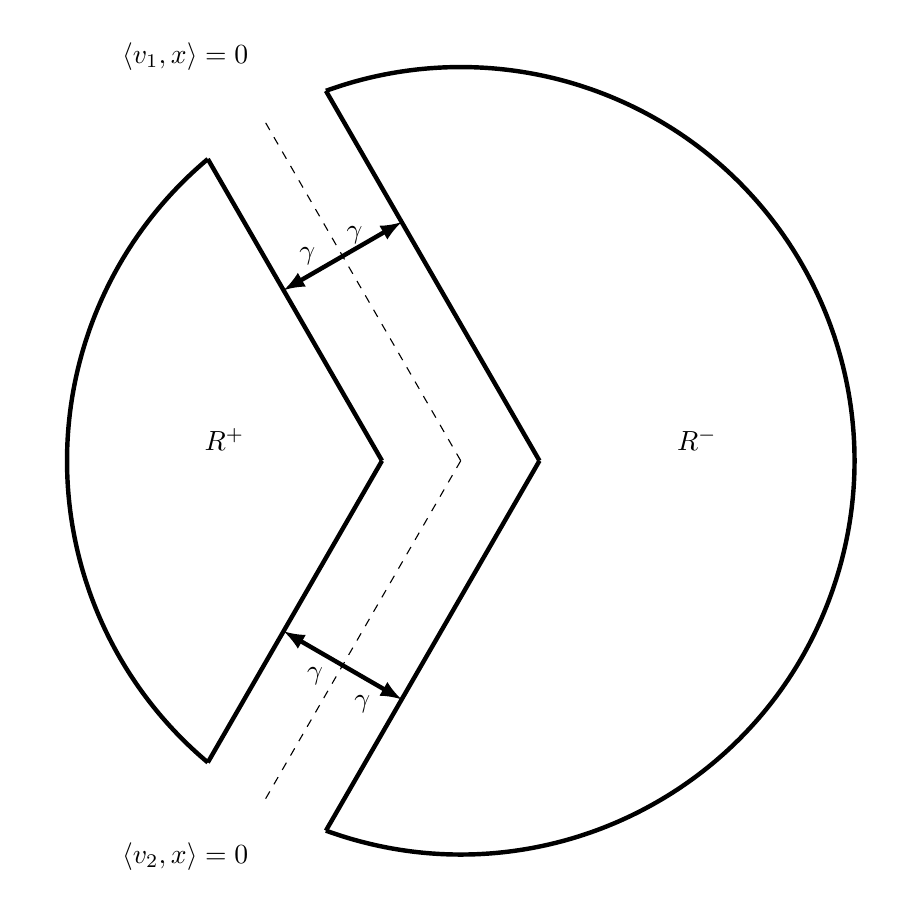
\begin{tikzpicture}

  \useasboundingbox (-5.5,-5.5) rectangle (5.5,5.5);
  % \draw[help lines] (-5.5,-5.5) rectangle (5.5,5.5);

  % Grid and coordinate axes
  %% \draw[help lines] (-5.2,-5.2) grid (5.2,5.2);
  %% \draw[thick, ->, >=latex] (-5.2,0) -- (5.2,0);
  %% \draw[thick, ->,  >=latex] (0,-5.2) -- (0,5.2);

  % Notable points
  \coordinate (Origin) at (0,0);

  \coordinate [label={[xshift=-10mm, yshift=5mm]$\ip{v_1}{x} = 0$}] (A) at (120:5);
  \coordinate [label={[xshift=-10mm, yshift=-10mm]$\ip{v_2}{x} = 0$}] (B) at (240:5);

  % Circle which contains all the examples.
  % \draw (Origin) circle (5cm);

  \draw[dashed] (Origin) -- (A);
  \draw[dashed] (Origin) -- (B);

  \coordinate (A1) at ($(120:0.5*sqrt{97} - 0.5) - (1,0)$);
  \coordinate (B1) at ($(240:0.5*sqrt{97} - 0.5) - (1,0)$);

  \coordinate (A2) at ($(120:0.5*sqrt{97} + 0.5) + (1,0)$);
  \coordinate (B2) at ($(240:0.5*sqrt{97} + 0.5) + (1,0)$);

  \draw[ultra thick] ($(Origin) - (1,0)$) -- (A1);
  \draw[ultra thick] ($(Origin) - (1,0)$) -- (B1);

  \draw[ultra thick] ($(Origin) + (1,0)$) -- (A2);
  \draw[ultra thick] ($(Origin) + (1,0)$) -- (B2);

  \pic [ultra thick, draw, angle radius=5cm] {angle=A1--Origin--B1};
  \pic [ultra thick, draw, angle radius=5cm] {angle=B2--Origin--A2};


  \coordinate (C) at (120:3);
  \coordinate [label={[xshift=-6mm, yshift=-4mm]$\gamma$}] (C1) at ($(120:3) + (0.75, 0.43301270189221932338)$);
  \coordinate [label={[xshift=+3mm, yshift=+2mm]$\gamma$}] (C2) at ($(120:3) - (0.75, 0.43301270189221932338)$);
  \draw[<->, >=latex, ultra thick] (C1) -- (C) -- (C2);

  \coordinate (D) at (240:3);
  \coordinate [label={[xshift=+4mm, yshift=-8mm]$\gamma$}] (D1) at ($(240:3) + (-0.75, 0.43301270189221932338)$);
  \coordinate [label={[xshift=-5mm, yshift=-3mm]$\gamma$}] (D2) at ($(240:3) - (-0.75, 0.43301270189221932338)$);
  \draw[<->, >=latex, ultra thick] (D1) -- (D) -- (D2);

  \coordinate [label={$R^+$}](R1) at ($(Origin) - (3,0)$);
  \coordinate [label={$R^-$}](R2) at ($(Origin) + (3,0)$);

\end{tikzpicture}

\end{center}
\caption[]{The figure shows the two regions used in parts 1 and 2 of
Theorems~\ref{theorem:polynomial-approximation-1}~and~\ref{theorem:polynomial-approximation-2}
for the case $m=d=2$ and a particular choice of vectors $v_1, v_2$ and margin
parameter $\gamma$. These regions are
$R^+ = \displaystyle \bigcap_{i=1}^m \left\{ x \in \R^d ~:~ \norm{x} \le 1, \ \ip{v_i}{x} \ge \gamma \right\}$,
$R^- = \displaystyle \bigcup_{i=1}^m \left\{ x \in \R^d ~:~ \norm{x} \le 1, \ \ip{v_i}{x} \le - \gamma \right\}$
The separating hyperplanes $\ip{v_1}{x} = 0$ and $\ip{v_2}{x} = 0$ are shown as dashed lines.}
\label{figure:pizza-slice}
\end{figure}

We construct the three different mappings $\phi_n, \psi_n, \rho$. The first two
are parameterized by a non-negative integer $n$. The domain of $\phi_n$ and
$\psi_n$ is $\R^d$. The domain of $\rho$ is the unit ball of $\R^d$. The
co-domain of $\phi_n$ and $\psi_n$ is $\R^q$ where $q = \sum_{i=0}^n
\binom{i+d-1}{d-1}$ equipped with the standard inner product $\ip{x}{x'}_{\R^q} =
\sum_{i=1}^p x_i x'_i$. The co-domain of $\rho$ is the classical real separable Hilbert space
$\ell_2 = \{ x \in \R^\infty ~:~ \sum_{i=1}^\infty x_i^2 < + \infty \}$ equipped
with the standard inner product $\ip{x}{x'}_{\ell_2} = \sum_{i=1}^\infty x_i x'_i$. We
index the coordinates of the co-domain $\R^q$ by $d$-tuples $(\alpha_1,
\alpha_2, \dots, \alpha_d)$ of non-negative integers such that $\alpha_1 +
\alpha_2 + \dots + \alpha_d \le n$. Similarly, we index the coordinates of
$\ell_2$ by $d$-tuples $(\alpha_1, \alpha_2, \dots, \alpha_d)$ of non-negative
integers. The mappings are defined by
\begin{align*}
& \left(\phi_n(x_1, x_2, \dots, x_d)\right)_{(\alpha_1, \alpha_2, \dots, \alpha_d)}
= x_1^{\alpha_1} x_2^{\alpha_2} \dots x_d^{\alpha_d}
\\
& \left(\psi_n(x_1, x_2, \dots, x_d)\right)_{(\alpha_1, \alpha_2, \dots, \alpha_d)} = x_1^{\alpha_1} x_2^{\alpha_2} \dots x_d^{\alpha_d} \\
& \qquad \cdot \sqrt{\binom{n}{\alpha_1 + \alpha_2 + \dots + \alpha_d} \binom{\alpha_1 + \alpha_2 + \dots + \alpha_d}{\alpha_1, \alpha_2, \dots, \alpha_d}}
\\
& \left(\rho(x_1, x_2, \dots, x_d)\right)_{(\alpha_1, \alpha_2, \dots, \alpha_d)} = x_1^{\alpha_1} x_2^{\alpha_2} \dots x_d^{\alpha_d} \\
& \qquad \cdot \sqrt{2^{-(\alpha_1 + \alpha_2 + \dots + \alpha_d)} \binom{\alpha_1 + \alpha_2 + \dots + \alpha_d}{\alpha_1, \alpha_2, \dots, \alpha_d}}
\end{align*}
where $\binom{\alpha_1 + \alpha_2 + \dots + \alpha_d}{\alpha_1, \alpha_2, \dots, \alpha_d} = \frac{(\alpha_1 + \alpha_2 + \dots + \alpha_d)!}{\alpha_1! \alpha_2! \dots \alpha_d!}$
is the multinomial coefficient and $\binom{n}{k} = \frac{n!}{(n-k)!k!}$ is the binomial coefficient.

Mappings $\psi_n$ and $\rho$ have simple-to-compute kernels
\begin{align*}
K_{\psi_n}(x,x') & = \ip{\psi_n(x)}{\psi_n(x')}_{\R^q} = \left( 1 + \ip{x}{x'} \right)^n \; , \\
K_{\rho}(x,x') & = \ip{\rho(x)}{\rho(x')}_{\ell_2} = \frac{1}{1 - \frac{1}{2}\ip{x}{x'}} \; .
\end{align*}
In passing we note that the formula for $K_\rho$ implies the mapping $\rho$ is
well defined. Indeed, since $K_{\rho}(x,x) < +\infty$ for any $x$ in the unit
ball of $\R^d$, it means that $\rho(x)$ indeed lies in $\ell_2$.

Any mutlivariate polynomial in the orginal space $\R^d$ can be expressed as a
linear function in the new feature spaces given by mappings $\phi_n, \psi_n,
\rho$. The following lemma bounds the norm of the linear function in the terms
of the norm of the polynomial. Recall that a linear function in a Hilbert space
$(H, \ip{\cdot}{\cdot}_H)$ has the form $\ip{c}{x}_H$ for some vector $c \in H$
and its norm is $\norm{c}_H = \sqrt{\ip{c}{c}}$.

\begin{lemma}[Norm bound]
\label{lemma:norm-bound}
Let $d \ge 1$ and $n \ge 0$ be integers and let $q = \sum_{i=0}^n \binom{i+d-1}{d-1}$.
Let $p:\R^d \to \R$ be a multivariate polynomial.
\begin{enumerate}
\item If $n \ge \deg(p)$ then there exists $c \in \R^q$ such that $p(x) = \ip{c}{\phi_n(x)}_{\R^q}$
and $\norm{c}_{\R^q} = \norm{p}$.
\item If $n \ge \deg(p)$ then there exists $c' \in \R^q$ such that $p(x) = \ip{c'}{\psi_n(x)}_{\R^q}$
and $\norm{c'}_{\R^q} \le \norm{p}$.
\item There exists $c'' \in \ell_2$ such that $p(x) = \ip{c''}{\psi_n(x)}_{\ell_2}$
and $\norm{c''}_{\R^q} \le 2^{\deg(p)/2} \norm{p}$.
\end{enumerate}
\end{lemma}

\begin{proof}
Note that the polynomial $p$ can be written as
$p(x) = \sum_{\alpha_1, \alpha_2, \dots, \alpha_d} c_{\alpha_1, \alpha_2, \dots, \alpha_d} x_1^{\alpha_1} x_2^{\alpha_2} \dots x_d^{\alpha_d}$.
There are $\sum_{i=0}^{\deg(p)} \binom{i+d-1}{d-1}$ coefficients $c_{\alpha_1, \alpha_2, \dots, \alpha_d}$.
If $n \ge \deg(p)$ these can be expressed as a vector in $c \in \R^q$. Thus, $p(x) = \ip{c}{\phi_n(x)}_{\R^q}$
and
$$
\norm{c}_{\R^p} = \sqrt{\sum_{\alpha_1, \alpha_2, \dots, \alpha_d} (c_{\alpha_1, \alpha_2, \dots, \alpha_d})^2} =  \norm{p} \; .
$$

We define $c' \in \R^q$ using the multi-index notation as
$$
c'_{\alpha_1, \alpha_2, \dots, \alpha_d}
= \frac{c_{\alpha_1, \alpha_2, \dots, \alpha_d}}{\sqrt{\binom{n}{\alpha_1 + \alpha_2 + \dots + \alpha_d} \binom{\alpha_1 + \alpha_2 + \dots + \alpha_d}{\alpha_1, \alpha_2, \dots, \alpha_d}}} \; .
$$
We have $\ip{c'}{\psi_n(x)}_{\R^q} = \ip{c}{\phi_n(x)}_{\R^q} = p(x)$. Since
$$
|c'_{\alpha_1, \alpha_2, \dots, \alpha_d}| \le |c_{\alpha_1, \alpha_2, \dots, \alpha_d}| \; ,
$$
we have $\norm{c'}_{\R^q} \le \norm{c}_{\R^q} = \norm{p}$.

Similarly, we define $c'' \in \ell_2$ using the multi-index notation as
$$
c''_{\alpha_1, \alpha_2, \dots, \alpha_d}
= \frac{c_{\alpha_1, \alpha_2, \dots, \alpha_d} 2^{(\alpha_1 + \alpha_2 + \dots + \alpha_d)/2}}{\sqrt{\binom{\alpha_1 + \alpha_2 + \dots + \alpha_d}{\alpha_1, \alpha_2, \dots, \alpha_d}}}
$$
for all tuples $(\alpha_1, \alpha_2, \dots, \alpha_d)$ such that $\alpha_1 + \alpha_2 + \dots + \alpha_d \le \deg(p)$.
Otherwise, we define $c''_{\alpha_1, \alpha_2, \dots, \alpha_d} = 0$. We have
$\ip{c''}{\rho(x)}_{\ell_2} = \ip{c}{\phi_n(x)}_{\R^q} = p(x)$. Since
\begin{align*}
|c''_{\alpha_1, \alpha_2, \dots, \alpha_d}|
& \le 2^{(\alpha_1 + \alpha_2 + \dots + \alpha_d)/2} |c''_{\alpha_1, \alpha_2, \dots, \alpha_d}| \\
& \le 2^{\deg(p)/2} |c''_{\alpha_1, \alpha_2, \dots, \alpha_d}| \; ,
\end{align*}
we have $\norm{c''}_{\ell_2} \le 2^{\deg(p)/2} \norm{c}_{\R^q} = 2^{\deg(p)/2} \norm{p}$.
\end{proof}

Using the lemma and the polynomial approximation theorems, we can prove
the mappings $\phi_n, \psi_n, \rho$ map any a weakly separable data
to a strongly separable data set.

\begin{theorem}
Let $(x_1, y_1), (x_2, y_2), \dots, (x_T, y_T) \in \R^d \times \{1,2,\dots,K\}$
labeled examples that are weakly linearly separable with margin $\gamma > 0$
such that $\norm{x_1}, \norm{x_2}, \dots, \norm{x_T} \le 1$. Then, the labeled
examples $(\rho(x_1), y_1), (\rho(x_2), y_2), \dots, (\rho(x_T), y_T)$ are
strongly linearly separable with margin
$$
\gamma' = \frac{1}{2\sqrt{K} \left(376 \lceil \log_2(2m) \rceil \cdot \left \lceil \sqrt{\frac{2}{\gamma}} \right \rceil \right)^{\frac{1}{2} \lceil \log_2(2m) \rceil \cdot \left \lceil \sqrt{\frac{2}{\gamma}} \right \rceil}}
$$
and $\norm{\rho(x_1)}_{\ell_2}, \norm{\rho(x_2)}_{\ell_2}, \dots, \norm{\rho(x_T)}_{\ell_2} \le 2$.
TODO
\end{theorem}

\begin{proof}
First osberve that for any $t=1,2,\dots,T$,
$$
\norm{\rho(x_t)}_{\ell_2} = K_{\rho}(x_t,x_t) = \frac{1}{1 - \frac{1}{2} \norm{x_t}^2} \le 2 \; .
$$

Since the examples $(x_1, y_1), (x_2, y_2), \dots, (x_T, y_T)$ are weakly linearly separable
with margin $\gamma$ there are vectors $w_1, w_2, \dots, w_K$ satisfying
\eqref{equation:weak-linear-separability-1} anf \eqref{equation:weak-linear-separability-2}.

Fix any $i \in \{1,2,\dots,K\}$. Consider the $K-1$ vectors
$(w_i - w_j)/2$ for $j \in \{1,2,\dots,K\} \setminus \{i\}$. Note that the vectors
have norm at most $1$.
\autoref{theorem:polynomial-approximation-1} implies that
there exists a polynomial $p_i:\R^d \to \R$ such
that
$$
\deg(p) = \lceil \log_2(2m) \rceil \cdot \lceil \sqrt{\frac{2}{\gamma}} \rceil \; ,
$$
for all $t=1,2,\dots,T$, if $y_t = i$ then $p_i(x_t) \ge 1/2$ and if $y_t \neq i$ then $p_i(x_t) \le -1/2$,
and
$$
\norm{p} \le \left(188 \lceil \log_2(2m) \rceil \cdot \left \lceil \sqrt{\frac{2}{\gamma}} \right \rceil \right)^{\frac{1}{2} \lceil \log_2(2m) \rceil
\cdot \left \lceil \sqrt{\frac{2}{\gamma}} \right \rceil} \; .
$$
By \autoref{lemma:norm-bound} there exists $c_i \in \ell_2$ such that
$\ip{c_i}{\rho(x)} = p(x)$ and
$$
\norm{c_i}_{\ell_2}
\le \left(376 \lceil \log_2(2m) \rceil \cdot \left \lceil \sqrt{\frac{2}{\gamma}} \right \rceil \right)^{\frac{1}{2} \lceil \log_2(2m) \rceil
\cdot \left \lceil \sqrt{\frac{2}{\gamma}} \right \rceil} \; .
$$
Define vector $u_i \in \ell_2$ as
$$
u_i = \frac{c_i}{\sqrt{K} \left(376 \lceil \log_2(2m) \rceil \cdot \left \lceil \sqrt{\frac{2}{\gamma}} \right \rceil \right)^{\frac{1}{2} \lceil \log_2(2m) \rceil
\cdot \left \lceil \sqrt{\frac{2}{\gamma}} \right \rceil}} \; .
$$

Then, $\norm{u_1}^2 + \norm{u_2}^2 + \dots + \norm{u_K}^2 \le 1$ and
for all $t=1,2,\dots,T$, $\ip{u_{y_t}}{x_t} \ge \gamma'$
and for all $j \in \{1,2,\dots,K\} \setminus \{y_t\}$,
$\ip{u_j}{x_t} \le - \gamma'$. In other words,
$(\rho(x_1), y_1), (\rho(x_2), y_2), \dots, (\rho(x_T), y_T)$ are
strongly linearly separable with margin $\gamma'$.
\end{proof}

\input{proofs-of-polynomial-approximation-theorems}
\section{Nearest neighbor algorithm}

TODO

\section{NP-hardness of the weak labeling problem}

Any algorithm for the bandit setting collects information in the form of so
called \emph{strongly labeled} and \emph{weakly labeled} examples.
Strongly-labeled examples are those for which we know the class label. Weakly
labeled example is an example for which we know that class label can be anything
except for a particular one class.

A natural strategy for each round is to find vectors $w_1, w_2, \dots, w_K$ that
linearly separate the examples seen in the previous rounds and use the vectors
to predict the label in the next round. More precisely, we want to find both the
vectors $w_1, w_2, \dots, w_K$ and label for each example consistent with its
weak and/or strong labels such that $w_1, w_2, \dots, w_K$ linearly separate the
labeled examples. We show this problem is NP-hard even for $K=3$.

Clearly, the problem is at least as hard as the decision version of the problem
where the goal is to determine if such vectors and labeling exist. We show that
this problem is NP-complete.

We use for $1,2,\dots,K$ for strong labels and $\overline{1}, \overline{2},
\dots, \overline{K}$ for weak labels. We adopt the convention that
$\overline{\overline{i}} = i$ for any positive integer $i$. Formally, the weak
labeling problem can be described as below:
\begin{figure}[H]
\begin{framed}
\begin{center}
    \textbf{Weak Labeling}
\end{center}
\textbf{Given:} Feature-label pairs $(x_1, y_1)$, $(x_2, y_2)$, \dots, $(x_T, y_T)$ in $\{0,1\}^d \times \{1,2,\dots, K, \overline{1}, \overline{2}, \dots, \overline{K}\}$. \\
\textbf{Question:} Do there exist $ w_1, w_2, \dots, w_K \in \R^d$ such that for all $t=1,2,\dots,T$,
\begin{align*}
& y_t \in \{1,2,\dots,K\} \Longrightarrow  \\
& \quad \forall i \in \{1,2,\dots,K\} \setminus \{y_t\} \quad \ip{w_{y_t}}{x_t}  > \ip{w_i}{x_t} \; , \\
& \text{and} \\
& y_t \in \{\overline{1}, \overline{2},\dots, \overline{K}\} \Longrightarrow \\
& \quad \exists i \in \{1,2,\dots,K\} \quad \ip{w_i}{x_t} > \ip{w_{\overline{y_t}}}{x_t} \; ?
\end{align*}
\end{framed}
\end{figure}

The hardness proof is based on a reduction from the set splitting problem, which
is proven to be NP-complete by Lovasz \cite{Garey-Johnson-1979}, to our weak
labeling problem. The reduction is adapted from \cite{Blum-Rivest-1993}.
\begin{figure}[H]
\begin{framed}
\begin{center}
    \textbf{Set Splitting}
\end{center}
\textbf{Given:} A finite set $S$ and a collection $C$ of subsets $c_i$ of $S$. \\
\textbf{Question:} Do there exist disjoint sets $S_1$ and $S_2$ such that $S_1 \cup S_2 = S$ and $\forall i, c_i\not\subseteq S_1$ or $c_i\not\subseteq S_2$?
\end{framed}
\end{figure}

Below we show the reduction. Suppose we are given an instance of the set
splitting problem
\begin{align*}
S & = \{1, 2, \dots, N\} \; , \\
C & = \{c_1, c_2, \dots, c_M\} \; .
\end{align*}

We create the weak labeling instance as follows. Let $d=N+1$ and $K=3$.
Define $\zero$ as the zero vector $(0,\dots,0)\in \R^N$ and $\e_i$ as the
$i$-th standard vector $(0,\dots, 1, \dots, 0)\in \R^N$). Then we include all
the following feature-label pairs:
\begin{itemize}
\item Type 1: $(x,y)=((\zero,1), 3)$,
\item Type 2: $(x,y)=((\e_i,1), \overline{3})$ for all $i \in \{1,2,\dots,N\}$,
\item Type 3: $(x,y)=\left(\left(\sum_{i\in c_j} \e_i, 1\right), 3\right)$ for all $j \in \{1,2,\dots,M\}$.
\end{itemize}

For example, if we have $S=\{1,2,3\}$, $C=\{c_1, c_2\}$, $c_1 = \{1,2\}$,
$c_2=\{2,3\}$, then we create the weak labeling sample set as:
\begin{multline*}
\{
((0,0,0,1),3), ((1,0,0,1),\overline{3}), ((0,1,0,1),\overline{3}), \\
((0,0,1,1),\overline{3}), ((1,1,0,1),3), ((0,1,1,1),3)
\} \; .
\end{multline*}
The following lemma shows that answering this weak labeling problem is
equivalent to answering the original set splitting problem.

\begin{lemma}
Any instance of the set splitting problem is a YES instance if and only if the
corresponding instance of the weak labeling problem (as described above) is a
YES instance.
\end{lemma}

\begin{proof}
$(\Longrightarrow)$ Let $S_1, S_2$ be the solution of the set splitting problem. Define
$$
w_1 = \left(a_1, a_2, \cdots, a_N, -\frac{1}{2}\right),
$$
where for all $i \in \{1,2,\dots,N\}$, $a_i=1$ if $i\in S_1$ and $a_i=-N$ if
$i\notin S_1$. Similarly, define
$$
w_2 = \left(b_1, b_2, \cdots, b_N, -\frac{1}{2}\right),
$$
where for all $i \in \{1,2,\dots,N\}$, $b_i=1$ if $i \in S_2$ and $b_i=-N$ if
$i\notin S_2$. Finally, define
$$
w_3 = (0,0,\cdots, 0),
$$
the zero vector. To see this is a solution for the weak labeling problem, we
verify separately for Type 1-3 samples defined above. For Type 1 sample, we have
$$
\ip{w_3}{x} = 0 > -\frac{1}{2} = \ip{w_1}{x}=\ip{w_2}{x}.
$$
For a Type 2 sample that corresponds to index $i$, we have either $i\in S_1$ or
$i\in S_2$ because $S_1\cup S_2 = \{1,2,\dots,N\}$ is guaranteed. Thus, either
$a_i=1$ or $b_i=1$. If $a_i=1$ is the case, then
$$
\ip{w_1}{x} = a_i - \frac{1}{2} = \frac{1}{2} > 0 = \ip{w_3}{x};
$$
similarly if $b_i=1$, we have $\ip{w_2}{x}>\ip{w_3}{x}$. \\ For a Type 3 sample
that corresponds to index $j$, Since $c_j \not\subset S_1$, there exists some
$i'\in c_j$ and $i'\notin S_1$. Thus we have $x_{i'}=1$, $a_{i'}=-N$, and
therefore
\begin{align*}
\ip{w_1}{x}
& = a_{i'}x_{i'} + \sum_{i\in \{1,2,\dots,N\} \setminus \{i'\}} a_ix_i - \frac{1}{2} \\
& \le -N + (N-1)-\frac{1}{2} \\
& < 0 = \ip{w_3}{x} \; .
\end{align*}
Because $c_j \not\subset S_2$ also holds, we also have
$\ip{w_2}{x}<\ip{w_3}{x}$. This direction is therefore proved. \\
\ \\
$(\Longleftarrow)$ Given the solution $w_1, w_2, w_3$ of the weak labeling problem, we define
\begin{align*}
S_1 &= \left\{i \in \{1,2,\dots,n\} ~:~ \ip{w_1-w_3}{(\e_i, 1)} > 0 \right\}, \\
S_2 &= \left\{i \in \{1,2,\dots,n\} ~:~ \ip{w_2-w_3}{(\e_i, 1)} > 0 \text{\ and\ } i\notin S_1 \right\}.
\end{align*}
It is not hard to see $S_1 \cap S_2 = \emptyset$ and $S_1\cup S_2 =
\{1,2,\dots,N\}$. The former is because $S_2$ only includes elements that are
not in $S_1$. For the latter, note that $(\e_i, 1)$ is the feature vector for
Type 2 samples. Because Type 2 samples all have label $\overline{3}$, for any $i
\in \{1,2,\dots,N\}$, one of the following must hold: $\ip{w_1-w_3}{(\e_i,
1)}>0$ or $\ip{w_2-w_3}{(\e_i, 1)}>0$. This implies $i\in S_1$ or $i\in S_2$.

Now we show $\forall j$, $c_j \not\subset S_1$ and $c_j \not\subset S_2$ by
contraction. Assume there exists some $j$ such that $c_j \subset S_1$. By our
definition of $S_1$, we have $\ip{w_1-w_3}{(\e_i, 1)} > 0$ for all $i\in c_j$.
Therefore,
\begin{align*}
\sum_{i\in c_j} \ip{w_1-w_3}{\left(\e_i, 1\right)}
& = \ip{w_1-w_3}{\left(\sum_{i\in c_j} \e_i, |c_j|\right)}  \\
& > 0.
\end{align*}
Because Type 1 sample has label $3$, we also have
$$
\ip{w_1-w_3}{\left(\zero, 1\right)} < 0.
$$
Combining the above two inequalities, we get
\begin{align*}
& \ip{w_1-w_3}{\left(\sum_{i\in c_j}\e_i, 1\right)} \\
& = \ip{w_1-w_3}{\left(\sum_{i\in c_j}\e_i, |c_j|\right)}  \\
& \qquad - (|c_j|-1)\ip{w_1-w_3}{\left(\zero, 1\right)} \\
& > 0 \; .
\end{align*}
Note that $\left(\sum_{i\in c_j}\e_i, 1\right)$ is a feature vector for Type 3
samples. Thus the above inequality contradicts that Type 3 samples have label 3.
Therefore, $c_j \not\subset S_1$. If we assume there exists some $c_j \subset
S_2$, same arguments apply and also lead to contradiction.
\end{proof}

\section{Mistake lower bound for ignorant algorithms}
\label{section:mistake-lower-bound-for-ignorant-algorithms}

In this section, we prove a mistake lower bound for a family of algorithms
called \textit{ignorant algorithms}. Ignorant algorithms ignore the examples on
which they make mistakes. This assumption seems strong, but as we will explain
below, it is actually natural, and several recently proposed bandit
classification algorithms that achieve $\sqrt{T}$ regret bounds belong to
this family, e.g., SOBA~\citep{Beygelzimer-Orabona-Zhang-2017},
OBAMA~\citep{Foster-Kale-Luo-Mohri-Sridharan-2018}. Also,
\textsc{Nearest-Neighbor Algorithm} (Algorithm~\ref{algorithm:nearest-neighbor})
presented in Appendix~\ref{section:nearest-neighbor-algorithm} is an ignorant
algorithm.

Under the assumption that the examples lie in in the unit ball of $\R^d$ and are
weakly linearly separable with margin $\gamma$, we show that any ignorant
algorithm must make at least $\Omega \left( \left(\frac{1}{160 \gamma}\right)^{(d-2)/4} \right)$
mistakes in the worst case. In other words, an algorithm that achieves a better
mistake bound cannot ignore examples on which it makes a mistake and it must
make a meaningful update on such examples.

To formally define ignorant algorithms, we define the conditional distribution
from which an algorithm draws its predictions. Formally, given an algorithm
$\calA$ and an adversarial strategy, we define
\begin{multline*}
p_t(y|x) = \\
\Pr[y_t = y ~|~ (x_1, y_1), (x_2, y_2) \dots, (x_{t-1}, y_{t-1}), x_t = x] \; .
\end{multline*}
In other words, in any round $t$, conditioned on the past $t-1$ rounds, the
algorithm $\calA$ chooses $y_t$ from probability distribution $p_t(\cdot|x_t)$.
Formally, $p_t$ is a function $p:\{1,2,\dots,K\} \times \R^d \to [0,1]$
such that $\sum_{y=1}^K p_t(y|x) = 1$ for any $x \in \R^d$.

\begin{definition}[Ignorant algorithm]
An algorithm $\calA$ for \textsc{Online Multiclass Linear Classification with
Bandit Feedback} is called \emph{ignorant} if for every $t=1,2,\dots,T$,
$p_t$ is determined solely by the sequence
$(x_{a_1}, y_{a_1}), (x_{a_2}, y_{a_2}), \dots, (x_{a_n}, y_{a_n})$
in the rounds $1 \le a_1 < a_2 < \dots < a_n < t$ in which
the algorithm makes a correct prediction.
\end{definition}

An equivalent definition of an ignorant algorithm is that the memory state of
the algorithm does not change after it makes a mistake. Equivalently,
the memory state of an ignorant algorithm is completely determined
by the sequence of labeled examples on which it made correct prediction.

To explain the definition, consider an ignorant algorithm $\calA$. Suppose that
on a sequence of examples $(x_1, y_1), (x_2, y_2), \dots, (x_{t-1}, y_{t-1})$
generated by some adversary the algorthm $\calA$ makes correct predictions in
rounds $a_1, a_2, \dots, a_n$ where $1 \le a_1 < a_2 < \dots < a_n < t$ and
errors on rounds $\{1,2,\dots,t-1\} \setminus \{a_1, a_2, \dots, a_n\}$. Suppose
that on another sequence of examples $(x_1', y_1'), (x_2', y_2'), \dots,
(x_{s-1}', y_{s-1}')$ generated by another adversary the algorithm $\calA$ makes
correct predictions in rounds $b_1, b_2, \dots, b_n$ where $1 \le b_1 < b_2 <
\dots < b_n < s$ and errors on rounds $\{1,2,\dots,s-1\} \setminus \{b_1, b_2,
\dots, b_n\}$. Futhermore, suppose
\begin{align*}
(x_{a_1}, y_{a_1}) &= (x'_{b_1}, y'_{b_1}) \; , \\
(x_{a_2}, y_{a_2}) &= (x'_{b_2}, y'_{b_2}) \; , \\
\vdots \\
(x_{a_n}, y_{a_n}) &= (x'_{b_2}, y'_{b_n}) \; .
\end{align*}
Then, the definition
\begin{multline*}
\Pr[y_t = y ~|~ (x_1, y_1), (x_2, y_2) \dots, (x_{t-1}, y_{t-1}), x_t = x] = \\
\Pr[y_t' = y ~|~ (x_1', y_1'), (x_2', y_2') \dots, (x_{t-1}', y_{t-1}'), x_t' = x] \; .
\end{multline*}
Note that the sequences $(x_1, y_1)$, $(x_2, y_2)$, $\dots$, $(x_{t-1},
y_{t-1})$ and $(x_1', y_1')$, $(x_2', y_2')$, $\dots$, $(x_{s-1}', y_{s-1}')$
might have different lengths and and $\calA$ might error in different sets of
rounds. As a special case, if an ignorant algorithm makes a mistake in round $t$
then $p_{t+1}=p_t$.

Our main result is the following lower bound on the expected number of mistakes
for ignorant algorithms.

\begin{theorem}[Mistake lower bound for ignorant algorithms]
\label{theorem:ignorant-lower-bound}
Let $\gamma \in (0,1)$ and let $d$ be a positive integer. Suppose $\calA$ is an
ignorant algorithm for \textsc{Online Multiclass Linear Classification with
Bandit Feedback}. There exists $T$ and an adversary that sequentially chooses
labeled examples $(x_1, y_1), (x_2, y_2), \dots, (x_T, y_T) \in \R^d\times
\{1,2\}$ such that the examples are strongly linearly separable with magin
$\gamma$ and $\norm{x_1}, \norm{x_2}, \dots, \norm{x_T} \le 1$, and the expected
number of mistakes made by $\calA$ is at least
$$
\frac{1}{10} \left(\frac{1}{160\gamma}\right)^{\frac{d-2}{4}} \; .
$$
\end{theorem}

Before proving the theorem, we need the following lemma.

\begin{lemma}
\label{lemma:embed_d_gamma}
Let $\gamma \in (0,\frac{1}{160})$, let $d$ be a positive integer and let $N = (\frac{1}{2\sqrt{40\gamma}})^{d-2}$.
There exist vectors $u_1, u_2, \dots, u_N, v_1, v_2, \dots, v_N \in \R^d$ such that for all $i, j \in \{1,2,\dots,N\}$,
\begin{align*}
\norm{u_i} & \le 1 \; , \\
\norm{v_j} & \le 1 \; , \\
\ip{u_i}{v_j} & \ge \gamma & & \text{if $i=j$,} \\
\ip{u_i}{v_j} & \le -\gamma & & \text{if $i \neq j$.}
\end{align*}
\end{lemma}

\begin{proof}
By Lemma 6 of~\citet{Long-1995}, there exists vectors $z_1, z_2, \dots, z_N \in
\R^{d-1}$ such that $\norm{z_1} = \norm{z_2} = \dots = \norm{z_N} = 1$ and the
angle between the vectors is $\measuredangle(z_i, z_j) \ge \sqrt{40 \gamma}$ for
$i \neq j$, $i,j \in \{1,2,\dots,N\}$. Since $\cos\theta \le 1-\theta^2/5$ for
any $\theta \in [-\pi,\pi]$, this implies that
\begin{align*}
\ip{z_i}{z_j} &= 1 && \text{if $i = j$,} \\
\ip{z_i}{z_j} &\le 1 - 8\gamma && \text{if $i \neq j$.}
\end{align*}

Define $v_i = (\frac{1}{2} z_i, \frac{1}{2})$, and $u_i = (\frac{1}{2} z_i,
-\frac{1}{2}(1-4\gamma))$ for all $i \in \{1,2,\dots,N\}$. It can be easily
checked that for all $i$, $\norm{v_i} \le 1$ and $\norm{u_i} \le 1$.
Additionally,
$$
\ip{u_i}{v_j} = \frac{1}{4} \ip{z_i}{z_j} - \frac {1-4\gamma} 4 \; .
$$
Thus,
\begin{align*}
\ip{u_i}{v_j} &\ge \gamma && \text{if $i=j$,} \\
\ip{u_i}{v_j} &\le -\gamma && \text{if $i \neq j$.}
\end{align*}
\end{proof}

\begin{proof}
We consider the strategy for the adversary described in
Algorithm~\ref{algorithm:adversary-strategy}.

\begin{algorithm}
\caption{\textsc{Adversary's strategy}}
\label{algorithm:adversary-strategy}
\textbf{Define} $T=N$ and $v_1, v_2, \dots, v_N$ as in Lemma~\ref{lemma:embed_d_gamma}.\\
\textbf{Define} $q_0=\frac{1}{\sqrt{T}}$. \\
\textbf{Initialize} $\textsc{phase}= 1$. \\
\For{$t=1,2,\dots,T$}{
    \If{$\textsc{phase}=1$}{
       \If{$p_t(1|v_t)\ge 1-q_0$}{
          $(x_t, y_t)\leftarrow (v_t, 1)$
        }
       \Else{
          $(x_t, y_t)\leftarrow (v_t, 2)$ \\
          $\textsc{phase}\leftarrow 2$
       }
    }
    \Else{
         $(x_t, y_t)\leftarrow (x_{t-1}, y_{t-1})$
    }
}
\end{algorithm}

Define the indicators
\begin{align*}
A_t &= \indicator{\forall \tau\le t, p_\tau(1|x_\tau)<1-q_0} \\
B_t &= \indicator{\exists \tau\le t, p_\tau(1|x_\tau)\ge 1-q_0
 \text{\ and\ } \forall s\in[\tau,t), \widehat y_s \neq y_s}.
\end{align*}
Then we have
\begin{align}
& \mathbf{E}\left[\sum_{t=1}^{T} \indicator{\widehat y_t\neq y_t}\right] \nonumber \\
& \ge \mathbf{E}\left[\sum_{t=1}^T \indicator{\widehat y_t\neq y_t}A_t\right] \nonumber \\
& \qquad + \mathbf{E}\left[\sum_{t=1}^T \indicator{\widehat y_t\neq y_t}B_t\right] \nonumber \\
& = \mathbf{E}\left[\sum_{t=1}^T \mathbf{E}_t\left[\indicator{\widehat y_t\neq y_t}A_t\right]\right] + \mathbf{E}\left[\sum_{t=1}^T B_{t+1}\right] \nonumber \\
& \ge \mathbf{E}\left[\sum_{t=1}^T q_0 A_t\right] + \mathbf{E}\left[\sum_{t=1}^T B_{t+1}\right],
\label{equation:mistake_lower_bound_temp}
\end{align}
where in the first inequality we use the fact that $A_t$ and $B_t$ cannot be $1$
simultaneously; in the equality, we use $B_{t+1}=B_t\indicator{\widehat y_t\neq
y_t}$ by $B_t$'s definition; in the last inequality we use the fact that when
$t\le N$ and $A_t=1$, it must be $y_t=1$ and $\Pr[\widehat
y_t=y_t]=p_t(1|x_t)<1-q_0$. Now, denote $T_1 = \argmin_{\tau} \{
p_\tau(1|x_\tau) \ge 1-q_0 \}$ (if such $\tau$ does not exist or is larger than
$T$, we simply let $T_1=T+1$). Then $A_t=1$ for all $t\le
T_1-1$.

Note that $B_{T_1}=1$, and for $t \ge T_1$ the adversary will switch to
``$\textsc{phase}=2$'' and has $y_t=2$. Therefore,
$\Exp[B_{t+1}=0|B_{t}=1]=\Pr[\widehat y_t=y_t~|~B_t=1] = \Pr[\widehat
y_t=2|B_t=1].$ Note that when $B_t=1$, by definition there exists a $\tau\le t$
with $p_\tau(1|x_\tau)\ge 1-q_0$, and the algorithm all makes mistakes at $\tau,
\tau+1, \ldots, t$. Since the algorithm is ignorant, and when
$\textsc{phase}=2$, the features all remain the same, we have
$p_t(1|x_t)=p_{t-1}(1|x_{t-1})=\cdots=p_\tau(1|x_\tau)\ge 1-q_0$. Thus we can
further upper bound $\Exp[B_{t+1}=0|B_{t}=1]$ by $\Pr[\widehat y_t=2|B_t=1]\leq
q_0$. Thus the second term in \eqref{equation:mistake_lower_bound_temp} can be
calculated as

\begin{align*}
\mathbf{E}\left[\sum_{t=1}^T B_{t+1}\right]
& \ge \mathbf{E}\left[\sum_{t=T_1}^T (1-q_0)^{t-T_1+1} \right] \\
& = \frac{1-q_0}{q_0}\mathbf{E}\left[1-(1-q_0)^{T - T_1 + 1}\right] \; .
\end{align*}
Combining \eqref{equation:mistake_lower_bound_temp} and the above inequalities, we get
\begin{multline}
\label{equation:mistake_lower_bound_temp2}
\mathbf{E} \left[\sum_{t=1}^T \indicator{\widehat y_t\neq y_t}\right] \ge
\\ \mathbf{E}\left[q_0(T_1-1)+\frac{1-q_0}{q_0}\left(1-(1-q_0)^{T-T_1+1}\right)\right].
\end{multline}
In the case $T_1\ge \frac{1}{2}T + 1$, the right-hand side of
\eqref{equation:mistake_lower_bound_temp2} is lower bounded by
$\frac{1}{2}q_0 T = \frac{1}{2} \sqrt{T}$. In the case
$T_1< \frac{1}{2}T+1$, it is lower bounded by
\begin{align*}
& \frac{1-q_0}{q_0}\left(1-(1-q_0)^{\frac{1}{2}T}\right) \\
& = \frac{1-q_0}{q_0}\left(1-(1-q_0)^{\frac{1}{2q_0^2}}\right) \\
& \ge \frac{1-\frac{1}{\sqrt{2}}}{q_0}\left(1-\frac{1}{\sqrt{e}}\right) \\
& \ge \frac{1}{10} \sqrt{T} \; .
\end{align*}

Observe that in phase 1, the labels are equal to $1$ and in phase 2 the labels
are equal to $2$. Let $t$ be the round in which the switch happens. (If it never
happens, define $t=T+1$.) Note that $(x_t, y_t)=(x_{t+1}, y_{t+1})= \dots =
(x_T, y_T) = (v_t, 2)$. Consider the vectors $u_1, u_2, \dots, u_N$ as defined
in Lemma~\ref{lemma:embed_d_gamma} We claim that $w_1=-u_t/2$ and $w_2=u_t/2$
satisfy the conditions of strong linear separabaility.

Clearly $\norm{w_1}^2 + \norm{w_2}^2 \le (\norm{w_1} + \norm{w_2})^2 \le
(\frac{1}{2} + \frac{1}{2})^2 \le 1$. By Lemma~\ref{lemma:embed_d_gamma}, we
have $\ip{w_2/2}{x_s} = \ip{u_t/2}{v_t} \ge \gamma/2, \forall s \ge t$ and
$\ip{w_2/2}{x_s} = \ip{u_t/2}{v_s} \le - \gamma/2$ for all $s<t$. Similarly,
$\ip{w_1/2}{x_s} \le -\gamma/2$ for all $s \ge t$ and $\ip{w_1/2}{x_s} \ge
\gamma/2$ for all $s < t$. Thus, the examples are strongly separable with margin
$\gamma$.
\end{proof}


\bibliographystyle{plainnat}
\bibliography{biblio}

\appendix

\section{Multiclass Perceptron}
\label{section:multiclass-perceptron-proofs}

\textsc{Multiclass Perceptron} is an algorithm for \textsc{Online Multiclass
Classification}. Both the protocol for the problem and the algorithm are stated
below. The algorithm assumes that the feature vectors come from an inner product
space $(V, \ip{\cdot}{\cdot})$.

Two results are folklore. The first result is
\autoref{theorem:multiclass-perceptron-mistake-upper-bound} which states that if
examples are linearly separable with margin $\gamma$ and examples have norm
at most $R$ then the algorithm makes at most $\lfloor 2 (R/\gamma)^2 \rfloor$
mistakes. The second result is
\autoref{theorem:online-multiclass-classification-mistake-lower-bound} which
states that under the same assumptions as in
\autoref{theorem:online-multiclass-classification-mistake-lower-bound}
\emph{any} deterministic algorithm for \textsc{Online Multiclass Classification}
must make at least $\lfloor (R/\gamma)^2 \rfloor$ mistakes in the worst case.

\begin{protocol}[h]
\caption{\textsc{Online Multiclass Classification}
\label{algorithm:mutliclass-classification}}
\textbf{Require:} Number of classes $K$, number of rounds $T$. \\
\textbf{Require:} Inner product space $(V,\ip{\cdot}{\cdot})$. \\
\For{$t=1,2,\dots,T$}{
Adversary chooses example $(x_t, y_t) \in V \times \{1,2,\dots,K\}$, where $x_t$ is revealed to the learner.\\
Predict class label $\widehat y_t \in \{1,2,\dots,K\}$.\\
Observe feedback $y_t$
}
\end{protocol}

\begin{algorithm}[h]
\caption{\textsc{Multiclass Perceptron}
\label{algorithm:mutliclass-perceptron}}
\textbf{Require:} Number of classes $K$, number of rounds $T$. \\
\textbf{Require:} Inner product space $(V,\ip{\cdot}{\cdot})$. \\
Initialize $w_1^{(1)} = w_2^{(1)} = \dots = w_K^{(1)} = 0$ \\
\For{$t=1,2,\dots,T$}{
  Observe feature vector $x_t \in V$ \\
  Predict $\widehat y_t = \argmax_{i \in \{1,2,\dots,K\}} \ip{w_t^{(i)}}{x_t}$ \\
  Observe $y_t \in \{1,2,\dots,K\}$ \\
  \If{$\widehat y_t \neq y_t$}{
    Set $w_i^{(t+1)} = w_i^{(t)}$ \\ \qquad for all $i \in \{1,2,\dots,K\} \setminus \{y_t, \widehat y_t\}$ \\
    Update $w_{y_t}^{(t+1)} = w_{y_t}^{(t)} + x_t$ \\
    Update $w_{\widehat y_t}^{(t+1)} = w_{\widehat y_t}^{(t)} - x_t$ \\
  }
  \Else{
    Set $w_i^{(t+1)} = w_i^{(t)}$ for all $i \in \{1,2,\dots,K\}$ \\
  }
}
\end{algorithm}

\begin{theorem}[Mistake upper bound~\cite{Crammer-Singer-2003}]
\label{theorem:multiclass-perceptron-mistake-upper-bound}
Let $(V, \ip{\cdot}{\cdot})$ be an inner product space, let $K$ be a positive
integer, let $\gamma$ be a positive real number and let $R$ be a non-negative real
number. If $(x_1, y_1), (x_2, y_2), \dots, (x_T, y_T)$ is a sequence of labeled
examples in $V \times \{1,2,\dots,K\}$ that are weakly linearly separable with margin
$\gamma$ and $\norm{x_1}, \norm{x_2}, \dots, \norm{x_T} \le R$
then \textsc{Multiclass Perceptron} algorithm makes at most $\lfloor
2(R/\gamma)^2 \rfloor$ mistakes.
\end{theorem}

\begin{proof}
Let $M = \sum_{t=1}^T \indicator{\widehat y_t \neq y_t}$ be the number of
mistakes the algorithm makes. Since the $K$-tuple $(w_1^{(t)}, w_2^{(t)}, \dots,
w_K^{(t)})$ changes only if a mistake is made, we can upper bound $\sum_{i=1}^K
\norm{w_i^{(t)}}^2$ in terms of number of mistakes.
If a mistake happens in round $t$ then
\begin{align*}
& \sum_{i=1}^K \norm{w_i^{(t+1)}}^2 \\
& = \left(\sum_{i \in \{1,2,\dots,K\} \setminus \{y_t, \widehat y_t\} } \norm{w_i^{(t)}}^2 \right) \\
& \qquad + \norm{w_{y_t}^{(t)} + x_t}^2 + \norm{w_{\widehat y_t}^{(t)} - x_t}^2 \\
& = \left(\sum_{i \in \{1,2,\dots,K\} \setminus \{y_t, \widehat y_t\} } \norm{w_i^{(t)}}^2 \right) + \norm{w_{y_t}^{(t)}}^2 + \norm{w_{\widehat y_t}^{(t)}}^2 \\
& \qquad + 2 \norm{x_t}^2 + 2 \ip{w_{y_t}^{(t)} - w_{\widehat y_t}^{(t)}}{x_t} \\
& = \left(\sum_{i=1}^K \norm{w_i^{(t)}}^2 \right) + 2 \norm{x_t}^2 + 2 \ip{w_{y_t}^{(t)} - w_{\widehat y_t}^{(t)}}{x_t} \\
& \le \left(\sum_{i=1}^K \norm{w_i^{(t)}}^2 \right) + 2 \norm{x_t}^2 \\
& \le \left(\sum_{i=1}^K \norm{w_i^{(t)}}^2 \right) + 2 R^2 \; .
\end{align*}
So each time a mistake happens, $\sum_{i=1}^K \norm{w_i^{(t)}}^2$ increases by at most $2R^2$. Thus,
$$
\sum_{i=1}^K \norm{w_i^{(T+1)}}^2 \le 2R^2 M \; .
$$
Let $w_1^*, w_2^*, \dots, w_K^* \in V$ be vectors satisfying the
\eqref{equation:weak-linear-separability-1} and
\eqref{equation:weak-linear-separability-2}. We lower bound $\sum_{i=1}^K \ip{w_i^*}{w_i^{(t)}}$. This quantity changes
only when a mistakes happens. If mistake happens in round $t$, we have
\begingroup
\allowdisplaybreaks
\begin{align*}
& \sum_{i=1}^K \ip{w_i^*}{w_i^{(t+1)}} \\
& = \left( \sum_{i \in \{1,2,\dots,K\} \setminus \{y_t, \widehat y_t\}} \ip{w_i^*}{w_i^{(t)}} \right) \\
& \qquad + \ip{w_{y_t}^*}{w_{y_t}^{(t)} + x_t} + \ip{w_{\widehat y_t}^*}{w_{\widehat y_t}^{(t)} - x_t} \\
& = \left( \sum_{i=1}^K \ip{w_i^*}{w_i^{(t)}} \right) + \ip{w_{y_t}^* - w_{\widehat y_t}^*}{x_t} \\
& \ge  \left( \sum_{i=1}^K \ip{w_i^*}{w_i^{(t)}} \right) + \gamma \; .
\end{align*}
\endgroup
Thus, after $M$ mistakes,
$$
\sum_{i=1}^K \ip{w_i^*}{w_i^{(T+1)}} \ge \gamma M \; .
$$
We upper bound the left hand side by using Cauchy-Schwartz inequality twice and
the condition \eqref{equation:weak-linear-separability-1} on $w_1^*, w_2^*, \dots,
w_K^*$. We have
\begin{align*}
\sum_{i=1}^K \ip{w_i^*}{w_i^{(T+1)}}
& \le \sum_{i=1}^K \norm{w_i^*} \cdot \norm{w_i^{(T+1)}} \\
& \le \sqrt{\sum_{i=1}^K \norm{w_i^*}^2} \sqrt{\sum_{i=1}^K \norm{w_i^{(T+1)}}^2} \\
& \le \sqrt{\sum_{i=1}^K \norm{w_i^{(T+1)}}^2} \; .
\end{align*}
Combining all inequalities, we get
$$
(\gamma M)^2 \le \sum_{i=1}^K \norm{w_i^{(T+1)}}^2 \le 2R^2 M \; .
$$
We conclude that $M \le 2(R/\gamma)^2$. Since $M$ is an integer, $M \le \lfloor 2(R/\gamma)^2 \rfloor$.
\end{proof}


\begin{theorem}[Mistake lower bound]
\label{theorem:online-multiclass-classification-mistake-lower-bound}
Let $K$ be a positive integer, let $\gamma$ be a positive real number and let
$R$ be a non-negative real number. For any (possibly randomized) algorithm
$\calA$ for the \textsc{Online Multiclass Classification} problem there exists
an inner product space $(V, \ip{\cdot}{\cdot})$, a non-negative integer $T$ and
a sequence of labeled examples $(x_1, y_1), (x_2, y_2), \dots, (x_T, y_T)$
examples in $V \times \{1,2,\dots,K\}$ that are weakly linearly separable with
margin $\gamma$, the norms satisfy $\norm{x_1}, \norm{x_2}, \dots, \norm{x_T}
\le R$ and the algorithm makes at least $\frac 1 2 \lfloor (R/\gamma)^2 \rfloor$
mistakes.
\end{theorem}

\begin{proof}
Let $T = \lfloor (R/\gamma)^2 \rfloor$, $V = \R^T$, and for all $t$ in
$\cbr{1,\ldots,T}$, define instance $x_t = R e_t$ where $e_t$ is $t$-th element
of the standard orthonormal basis of $\R^T$.
Let labels $y_1, \ldots, y_T$ be chosen i.i.d uniformly at random from
$\cbr{1,2,\ldots,K}$ and independently of any randomness used by the algorithm
$\calA$.


%let $x_1, x_2, \dots, x_T$ be the
%orthogonal vectors such that $\norm{x_t} = R$ for all $t=1,2,\dots,T$. For
%example, we can take

%Since the algorithm is deterministic, we can construct the sequence of labels
%$y_1, y_2, \dots, y_T$ adaptively based on the predictions $\widehat y_1,
%\widehat y_2, \dots, \widehat y_T$ of the algorithm. We define $y_t$ to be any
%element of $\{1,2,\dots,K\}$ not equal to $\widehat y_t$. This way the algorithm
%makes a mistake in every round $t=1,2,\dots,T$.

We first show that the set of examples $(x_1,y_1)$, $\ldots$,
$(x_T, y_T)$ we have constructed is weakly linearly separable
with margin $\gamma$. To prove that, we demonstrate vectors $w_1, w_2, \dots, w_K$
satisfying conditions \eqref{equation:weak-linear-separability-1} and
\eqref{equation:weak-linear-separability-2}. We define
$$
w_i = \frac{\gamma}{R} \sum_{\substack{t : 1 \le t \le T \\ y_t = i}} e_t \qquad \text{for $i=1,2,\dots,K$.}
$$
Let $a_i = |\{ t ~:~ 1 \le t \le T, \ y_t = i \}|$ be the number of occurrences of label $i$.
It is easy to see that
$$
\norm{w_i}^2 = \frac{\gamma^2}{R^2} \sum_{\substack{t : 1 \le t \le T \\ y_t = i}} \norm{e_t}^2 = \frac{a_i \gamma^2}{R^2} \qquad \text{for $i=1,2,\dots,K$.}
$$
Since $\sum_{i=1}^K a_i = T$,
$\sum_{i=1}^K \norm{w_i}^2 = T \cdot \frac{\gamma^2}{R^2} \leq 1$, i.e.
the condition
\eqref{equation:weak-linear-separability-1} holds. To verify condition
\eqref{equation:weak-linear-separability-2} consider any labeled example $(x_t,
y_t)$. Then, for any $i$ in $\cbr{1,\ldots,K}$, by the definition of $w_i$, we have
\begin{align*}
\ip{w_i}{x_t}
& = \frac{\gamma}{R} \sum_{\substack{s : 1 \le s \le T \\ y_s = i}} \ip{e_s}{R e_t} \\
& = \gamma \cdot \sum_{\substack{s : 1 \le s \le T \\ y_s = i}} \indicator{s = t} \\
& = \gamma \cdot \indicator{y_t = i}
\; .
\end{align*}
Therefore, if $i = y_t$, $\ip{w_i}{x_t} = \gamma$;
otherwise $i \neq y_t$, in which case $\ip{w_i}{x_t} = 0$.
Hence, condition \eqref{equation:weak-linear-separability-2} holds.

We now give a lower bound on the number of mistakes $\calA$ makes.
As $y_t$ is chosen uniformly from $\{1,2,\dots,K\}$ and independent of
$\calA$'s randomization
$$
\Exp[ \indicator{\widehat y_t \neq y_t} ] \ge 1 - \frac{1}{K} \ge \frac{1}{2} \; .
$$
Summing over all $t$ in $\cbr{1,\ldots,T}$, we conclude that
$$
\Exp \sbr{ \sum_{t=1}^T \indicator{\widehat y_t \neq y_t} } \geq \frac T 2 = \frac 1 2 \lfloor (R/\gamma)^2 \rfloor,
$$
which completes the proof.
\end{proof}

%& = \frac{R}{\sqrt{T}} \\
%& \ge \frac{R}{R/\gamma} \\
%& = \gamma \; .
%and similarly, for any $i \in \{1,2,\dots,K\} \setminus \{y_t\}$ we have
%$\ip{w_i}{x_t} = 0$.


\end{document}
